\chapter{Interprétation statistique - Limites d'exclusion}
\label{chap:interpretationStatLimit}

Les recherches de processus rares (que ce soit des processus de nouvelle physique ou des processus pr\'edits par le mod\`ele standard non encore observ\'es) se soldent malheureusement la plupart du temps par la non-observation du processus recherché. Ces r\'esultats, bien que moins d\'eterminant que des observations, permettent quand m\^eme d'apprendre quelque chose sur la physique des particules puisqu'ils peuvent \^etre utilis\'es pour contraindre les mod\`eles pr\'edisant ces processus. 

Une partie de mon travail entre 2012 et 2014 a porté sur le calcul de limites d'exclusion et le développement d'outils permettant ces calculs. 
Afin de comprendre ces travaux, pr\'esent\'es dans les chapitres \ref{chap:OTHandTIFOSI} et \ref{chap:Recherche4tops}, nous donnons dans ce chapitre un bref aper\c cu des m\'ethodes statistiques utilis\'ees en physique des particules. 
Un r\'esultat original sur l'\'equivalence entre l'approche hybride fr\'equentiste-bay\'esienne et l'approche bay\'esienne est \'egalement pr\'esent\'e. 

%les interpr\'etations statistiques r\'ealis\'ees pour la recherche d'\'ev\'enements avec quatre quarks top (pr\'esent\'ees dans le chapitre~\ref{chap:Recherche4tops}) et les outils d\'evelopp\'es (pr\'esent\'es dans le chapitre \ref{chap:OTHandTIFOSI}), 
%Les outils d\'evelopp\'es sont d\'ecrits dans le chapitre suivant.

\section{Généralités}
\label{sec:GeneraliteStat}

L'objectif d'une analyse en physique des particules est en général de construire des lots d'événements enrichis en événements de signal et appauvris en événements de bruit de fond, à partir desquels une inférence portant sur un ou plusieurs paramètres de la théorie sous-jacente peut être faite. Les observables mesurées sont les nombres d'événements dans chaque lot et, éventuellement, des variables caractérisant la cinématique ou la topologie des événements présentant un pouvoir discriminant entre le signal et les bruits de fond. Notons $X$ l'ensemble de ces observables et $x$ les valeurs qu'elles peuvent prendre. La loi de probabilité décrivant ces observables peut s'écrire, d'une manière générale, comme ceci :
\begin{equation}
\label{eq:loiProbaGenerale}
f_X(x;\theta,\nu)
\end{equation}
où $\theta$ représente les paramètres d'intérêt (c'est-à-dire ceux sur lesquels l'inférence porte) et $\nu$ les paramètres de nuisance (c'est-\`a-dire tous les param\`etres autres que les param\`etres d'int\'er\^et). En fonction de la nature des observables $X$, $f$ peut être soit une loi discrète, soit une loi continue, soit un mélange des deux. Sa forme exacte dépend du problème considéré.

Bien que $X$ d'un côté et $\theta$ et $\nu$ de l'autre représentent des grandeurs physiquement différentes, $f$ est en toute généralité une fonction de toutes ces grandeurs. Il est d'usage d'appeler $f$ la loi de probabilité (ou densit\'e de probabilit\'e si $X$ est continue ou fonction de masse si $X$ est discret) lorsqu'elle est vue comme une fonction de $X$ avec $\theta$ et $\nu$ fixes et la fonction de vraisemblance lorsqu'elle est vue comme une fonction de $\theta$ et $\nu$ avec $X$ fixe. Dans la suite nous ne ferons pas cette distinction et utiliserons tout le temps le terme de fonction de vraisemblance. Il devrait être clair, en fonction du contexte, si c'est $X$ ou $\theta$ et $\nu$ qui sont considérés comme fixes. De plus, afin d'alléger les notations nous la noterons $\Lh(\theta,\nu)$ ou plus simplement \mbox{$\Lh=\Lh(\theta,\nu)=f_X(x;\theta,\nu)$}.

Une attention particulière sera portée dans ce chapitre au cas des expériences de comptage car c'est ce type d'exp\'erience qui sera pr\'esent\'e dans le chapitre~\ref{chap:Recherche4tops}. 
Dans une expérience de comptage, la seule observable est le nombre d'événements et sa loi de probabilité est la loi de Poisson. Si plusieurs canaux d'analyse indépendants sont considérés la fonction de vraisemblance s'écrit, en notant $N_c$ le nombre d'événements dans le canal $c$,
\begin{equation}
\label{eq:poissonLikelihoodGeneral}
\Lh=\prod\limits_c\left[\frac{\lambda_c(\theta,\nu)^{\nc}}{\nc!}e^{-\lambda_c(\theta,\nu)}\right]
\end{equation} 
où $\lambda_c$ est le nombre d'événements attendu dans le canal $c$, fonction des paramètres d'intérêt et de nuisance. $\lambda_c$ est la somme d'une contribution de signal et d'une ou plusieurs contributions de bruit de fond. De plus, dans les cas que nous considérerons par la suite, le seul paramètre d'intérêt sera l'intensité du signal $\mu=\sigma/\sigma_\text{ref}$, o\`u $\sigma$ est la section efficace et $\sigma_\text{ref}$ une section efficace de r\'ef\'erence (correspondant le plus souvent \`a la section efficace pr\'edite par le mod\`ele). Nous pouvons donc r\'eécrire l'équation \ref{eq:poissonLikelihoodGeneral} comme ceci :
\begin{equation}
\label{eq:poissonLikelihoodExplicitSigBkg}                                                                                                        
\Lh\left(\mu,\nu\right)=\prod\limits_c\left[\frac{\left(\mu \scc(\nu)+\sum\limits_i \bci(\nu)\right)^{\nc}}{\nc!}e^{-\left(\mu \scc(\nu)+\sum\limits_i \bci(\nu)\right)}\right]
\end{equation}
où $\scc$ et $\bci$ sont les nombres d'événements de signal et de bruit de fond de type $i$ attendus dans le canal $c$. Il est important de noter que ces nombres ne dépendent que des paramètres de nuisance (s'il y en a), le param\`etre d'int\'er\^et ayant \'et\'e isol\'e. 

Dans le cas où les nombres d'événements attendus de signal et de bruit de fond sont parfaitement connus, $\scc$ et $\bci$ sont des constantes. La plupart du temps nous ne nous trouvons malheureusement pas dans ce cas. Ils varient sous l'effet de différentes sources d'incertitude. Par exemple, ils peuvent dépendre de l'échelle en énergie des jets qui n'est connue que de manière approximative ou de la section efficace d'un bruit de fond qui est entachée d'une erreur. Les paramètres de nuisance permettent de décrire ces dépendances pour chaque source d'incertitude. Une des limitations des analyses actuelles est que, pour chaque source d'incertitude, seuls trois points sont utilisés pour construire les fonctions $\scc(\nu)$ et $\bci(\nu)$ : les valeurs nominales et les valeurs obtenues en faisant varier les sources d'incertitudes de $\pm 1\sigma$. Entre ces trois points il est nécessaire d'interpoler et au-delà d'extrapoler. Ces interpolations et extrapolations sont dans une grande mesure arbitraires. Nous verrons dans le chapitre~\ref{chap:OTHandTIFOSI} que les outils que nous avons développé proposent différentes configurations permettant d'évaluer la dépendance des résultats à ces choix.

Bien qu'incertaines, les valeurs des nombres d'événements attendus de signal et de bruit de fond ne sont en général pas équiprobables. Elles sont en effet la plupart du temps contraintes soit par des mesures soit par des calculs théoriques effectués préalablement à la mesure principale décrite par l'équation~\ref{eq:poissonLikelihoodExplicitSigBkg}. La signification précise de ces contraintes et la fa\c con dont elles interviennent dans le processus d'inférence dépend de l'approche utilisée (fréquentiste, bayésienne ou hybride). Dans tous les cas, la fonction de vraisemblance complète incluant les termes de contrainte peut s'écrire
\begin{equation}
\label{eq:poissonLikelihoodExplicitSigBkgWithConstraint}                                                                                                        
\Lh\left(\mu,\nu\right)=\prod\limits_c\left[\frac{\left(\mu \scc(\nu)+\sum\limits_i \bci(\nu)\right)^{\nc}}{\nc!}e^{-\left(\mu \scc(\nu)+\sum\limits_i \bci(\nu)\right)}\right]g\left(\nu\right)
\end{equation}
où $g$ est le terme de contrainte des paramètres de nuisance. Dans la suite nous considérerons le cas où les paramètres de nuisance sont associés à des sources d'incertitudes indépendantes. $g$ s'écrira donc comme le produit des termes de contrainte associés à chaque source incertitude :
\begin{equation}
\label{eq:constrainFactorization}
g\left(\nu\right)=\prod\limits_j g_j(\nu_j)
\end{equation}
où $\nu_j$ est le paramètre de nuisance associé à l'incertitude $j$ et $g_j$ son terme de contrainte.

Les approches fréquentiste, bayésienne et hybride pour le calcul de limites d'exclusion sur le paramètre $\mu$ sont discutées brièvement dans la section suivante. Nous ne considérerons que le cas des expériences de comptage et donc des fonctions de vraisemblance ayant la forme donnée dans l'équation~\ref{eq:poissonLikelihoodExplicitSigBkgWithConstraint}. 

%Paramètres de nuisance \\
%  -> cas le plus simple : yields signal et bruit de fond sont des paramètres de nuisance\\
%      interpolation/extrapolation (ideal serait de faire des mesures à plusieurs valeurs de sigma mais impossible en pratique -> interpolation/extrapolation)\\
%  -> cas réaliste : plusieurs canaux, fonds et plusieurs incertitudes, possiblement correlées entre fonds/canaux.  \\
%
%Terme appelés de manière générale termes de contraintes\\

\section{Aper\c cu de différentes approches pour le calcul de limites d'exclusion}

Les diff\'erentes approches utilis\'ees en physique des particules pour calculer des limites d'exclusion sont d\'ecrites dans ce chapitre. Nous nous int\'eressons aux exp\'eriences de comptages d\'ecrites par l'\'equation \ref{eq:poissonLikelihoodExplicitSigBkgWithConstraint} o\`u $g\left(\nu\right)$ est donn\'e par l'équation~\ref{eq:constrainFactorization}. Les limites d'exclusion portent sur $\mu$ ou, de mani\`ere \'equivalente, sur la section efficace du processus recherch\'e.
 
Calculer une limite d'exclusion sur $\mu$ consiste \`a construire un intervalle de valeurs probables pour ce param\`etre born\'e inf\'erieurement par 0 et sup\'erieurement par la limite d'exclusion. Celle-ci sera not\'ee $\mup$. Nous cherchons donc \`a construire des intervalles de la forme 
\begin{equation}
\label{eq:limitInterval}
\left[0;\mup\right]
\end{equation}
ayant une grande probabilit\'e de contenir $\mu$, le sens exact assign\'e \`a "grande probabilit\'e" d\'ependant de l'approche statistique utilis\'ee.
%et sera pr\'ecis\'e, pour chacune d'elle, dans les sections suivantes. 

\subsection{Approche fréquentiste}

\subsubsection{Description}

Dans l'approche fréquentiste, $\mup$ est calculé en réalisant des tests d'hypothèses standards \cite{Stuart:436225}. Le test statistique utilis\'e est bas\'e sur la vraisemblance profil\'ee :
\begin{equation}
\label{eq:profileLikelihoodRatio}
\qmu=\left\{
\begin{tabular}{c l}
$-2\ln\displaystyle\frac{\Lh\left(\mu,\EstCond{\nu}\right)}{\Lh\left(\Est{\mu},\Est{\nu}\right)}$ & \text{si $\mu\geq\Est{\mu}$} \\
$0$ & \text{si $\mu < \Est{\mu}$}.
\end{tabular}
\right.
\end{equation}
o\`u $\Est{\mu}$ et $\Est{\nu}$ sont les estimateurs par maximum de vraisemblance de $\mu$ et $\nu$, et $\EstCond{\nu}$ est l'estimateur par maximum de vraisemblance conditionnel, calcul\'e en fixant $\mu$ \`a la valeur test\'ee ($\EstCond{\nu}$ est donc une fonction de $\mu$ : $\EstCond{\nu}=\EstCond{\nu}\left(\mu\right)$). L'hypoth\`ese nulle est l'hypoth\`ese signal plus bruit de fond ($\mu>0$) et l'hypoth\`ese alternative est l'hypoth\`ese bruit de fond seul ($\mu=0$). L'hypoth\`ese nulle est test\'ee pour plusieurs valeurs de $\mu$. L'intervalle de confiance donn\'e par l'équation~\ref{eq:limitInterval} est compos\'e de toutes les valeurs de $\mu$ pour lesquelles l'hypoth\`ese nulle n'est pas rejet\'ee. 

Dans l'\'equation~\ref{eq:profileLikelihoodRatio}, le test est pris \'egal \`a 0 lorsque $\mu<\Est{\mu}$ car les donn\'ees qui pr\'esentent une fluctuation du nombre d'\'ev\'enements vers le haut ne doivent pas \^etre consid\'er\'ees comme incompatibles avec l'hypoth\`ese $\mu$. Elle ne doivent donc pas faire partie de la r\'egion critique\footnote{La r\'egion critique est la r\'egion dans l'espace des observables qui conduit au rejet de l'hypoth\`ese nulle.} (une limite sup\'erieure correspond \`a un intervalle de confiance unilat\'eral et doit donc \^etre bas\'e sur un test d'hypoth\`ese unilat\'eral).  

Dans l'approche fr\'equentiste de base, l'hypoth\`ese nulle est rejet\'ee si
\begin{equation}
\label{eq:inequalityCLsb}
P\left(\qmu\geq\qmuobs|\mu'=\mu\right)<\alpha
%\displaystyle\int\limits_{\qmuobs}^{\infty}f\left(\qmu|\mu'=\mu\right)\dd\qmu < \alpha
\end{equation}
o\`u le membre de gauche est la probabilit\'e pour que \qmu~soit sup\'erieur \`a la valeur observ\'ee \qmuobs~sous l'hypoth\`ese $\mu'$ et $\alpha$ est l'erreur de premi\`ere esp\`ece. $1-\alpha$ est le niveau de confiance (ou CL pour \english{Confidence Level}). La valeur $\alpha=0,05$ est traditionnellement choisie, ce qui conduit \`a un niveau de confiance de 95\%. La limite sup\'erieure sur $\mu$ est donc solution de
\begin{equation}
\label{eq:CLsbDefOfMup}
P\left(\qmup\geq\qmupobs|\mu'=\mup\right)=\alpha
%\displaystyle\int\limits_{\qmupobs}^{\infty}f\left(\qmup|\mu'=\mup\right)\dd\qmup = \alpha
\end{equation}

La probabilit\'e dans les équations~\ref{eq:inequalityCLsb} et \ref{eq:CLsbDefOfMup} est commun\'ement appel\'ee \CLsb. Cette m\'ethode de calcul de limite d'exclusion est par cons\'equent appel\'ee "m\'ethode \CLsb". 

Un probl\`eme avec la m\'ethode \CLsb~est qu'elle peut conduire \`a rejeter des valeurs de $\mu$ inf\'erieures \`a 0 lorsque le nombre d'\'ev\'enements observ\'e est trop petit par rapport au nombre attendu. Ceci n'est pas physique et, pour pallier ce probl\`eme, les physiciens des particules utilisent depuis les exp\'eriences du LEP la m\'ethode dite \CLs~\cite{0954-3899-28-10-313}. Elle consiste \`a modifier l'équation~\ref{eq:CLsbDefOfMup} en divisant le membre de gauche par 
\begin{equation}
\label{eq:CLbdefinition}
\CLb=P\left(\qmu\geq\qmuobs|\mu'=0\right)
\end{equation}

La limite d'exclusion $\mup$ est donc telle que
\begin{equation}
\label{eq:CLsDefOfMup}
\CLs\left(\mup\right)=\alpha
\end{equation}
o\`u $\CLs=\CLsb/\CLb$ (la d\'ependance en $\mu$ a \'et\'e explicit\'ee dans l'équation~\ref{eq:CLsDefOfMup} pour plus de clart\'e).

\subsubsection{Limite asymptotique}
\label{sec:limiteAsymptotique}

Un des avantages de l'approche fr\'equentiste bas\'ee sur la vraisemblance profil\'ee donn\'ee dans l'\'equation~\ref{eq:profileLikelihoodRatio} est que la distribution de $\qmu$ est connue dans la limite asymptotique\footnote{La limite asymptotique est la limite lorsque la taille de l'\'echantillon de donn\'ees tend vers l'infini.}. En effet, dans cette limite nous avons (ce r\'esultat, d\^u \`a A. Wald \cite{Wald43}, est largement discut\'e dans~\cite{Stuart:436225})
\[-2\ln\displaystyle\frac{\Lh\left(\mu,\EstCond{\nu}\right)}{\Lh\left(\Est{\mu},\Est{\nu}\right)} \simeq \displaystyle\frac{\left(\mu-\Est{\mu}\right)^2}{\sigma^2}\]
o\`u $\Est{\mu}$ est distribu\'e suivant une loi normale d'esp\'erance $\mu'$ et d'\'ecart-type $\sigma$. $-2\ln\left(\Lh\left(\mu,\EstCond{\nu}\right)/\Lh\left(\Est{\mu},\Est{\nu}\right)\right)$ est donc distribu\'e suivant une loi de chi-carr\'e non centr\'ee. La fonction de r\'epartition de $\qmu$ est~\cite{2011EPJC...71.1554C} :
\[F\left(\qmu|\mu'\right) = \Phi\left(\sqrt{\qmu}-\displaystyle\frac{\mu-\mu'}{\sigma}\right)\]
o\`u $\Phi$ est la fonction de r\'epartition de la loi normale centr\'ee r\'eduite. \`A partir de cette expression nous pouvons d\'eduire la limite d'exclusion. En utilisant la m\'ethode \CLs{}, nous trouvons
\begin{equation}
\label{eq:pureFreqAsymptoticLimit}
\mup=\Est{\mu}+\sigma\Phi^{-1}\left[1-\alpha\times\Phi\left(\frac{\Est{\mu}}{\sigma}\right)\right]
\end{equation}



\subsubsection{Traitement des incertitudes}
\label{sec:frequentistTreatmentOfUncerts}

Le traitement des incertitudes (c'est-\`a-dire le sens donn\'e aux param\`etres de nuisance et leur traitement dans le calcul de limites) dans l'approche fr\'equentiste repose sur la notion d'exp\'erience auxiliaire. Les exp\'eriences auxiliaires sont les exp\'eriences au cours desquelles les incertitudes sur les sources incertitudes dans l'expérience principale sont estim\'ees. Afin d'illustrer cette notion, consid\'erons le cas d'une analyse dans laquelle une source d'incertitude est l'\'echelle en \'energie des jets. Les nombres d'\'ev\'enements attendus de signal et de bruit de fond sont donc fonction de l'\'echelle en \'energie des jets. Cette \'echelle en \'energie n'est pas inconnue. Elle a \'et\'e mesur\'ee dans \ATLAS~avec une certaine pr\'ecision gr\^ace \`a des m\'ethodes telles que celles pr\'esent\'ees dans le chapitre \ref{chap:calibjets}. Les nombres d'\'ev\'enements de signal et de bruit de fond attendus sont donc bien susceptibles de varier mais pas de mani\`ere arbitrairement grande. Leurs variations sont contraintes par la mesure qui a \'et\'e faite de l'incertitude sur l'\'echelle en \'energie des jets. Cette mesure est un exemple d'exp\'erience auxiliaire.

Ce qui vient d'\^etre dit sur l'\'echelle en \'energie des jets vaut \'egalement pour les autres sources d'incertitudes consid\'er\'ees typiquement dans les analyses de physique : \'echelle en \'energie des leptons, r\'esolution des jets et leptons, efficacit\'e d'\'etiquetage des jets provenant de quarks $b$, sections efficaces des bruits de fond, luminosit\'e, etc. Chacune de ces sources d'incertitude a fait l'objet d'une exp\'erience auxiliaire dont le r\'esultat peut \^etre utilis\'e dans l'expérience principale.

\`A chaque source d'incertitude est associ\'ee une observable qui est mesur\'ee dans l'exp\'erience auxiliaire correspondante. Notons $a_j$ ces observables ($j$ est un indice qui d\'esigne, comme dans la section~\ref{sec:GeneraliteStat}, la source d'incertitude). Chaque observable est d\'ecrite par une loi de probabilit\'e et ce sont ces lois de probabilit\'e qui sont utilis\'ees pour contraindre les param\`etres de nuisance $\nu_j$. 

Ce qui vient d'\^etre dit permet de donner un sens pr\'ecis aux termes $g_j$ dans l'\'equation~\ref{eq:constrainFactorization}. Nous voyons en effet que ces termes sont les fonctions de vraisemblance des exp\'eriences auxiliaires. Il serait plus correct de les \'ecrire $g_j\left(a_j;\nu_j\right)$ pour faire appara\^itre clairement que les $\nu_j$ sont des param\`etres et non des variables al\'eatoires (celles-ci \'etant les observables $a_j$). La fonction de vraisemblance globale donn\'ee dans l'\'equation~\ref{eq:poissonLikelihoodExplicitSigBkgWithConstraint} doit donc \^etre vue comme une fonction de vraisemblance conjointe, correspondant au produit des fonctions de vraisemblance associ\'ees 
\begin{maliste}
\item \`a l'exp\'erience principale (dans laquelle les nombres d'\'ev\'enements dans les diff\'erents canaux sont mesur\'es) et
\item aux exp\'eriences auxiliaires.
\end{maliste}

\subsubsection{Cas des incertitudes statistiques}
\label{sec:frequentistTreatmentOfStatUncert}

Les calculs des nombres d'\'ev\'enements de signal et de bruit de fond attendus sont souvent entach\'es d'incertitudes li\'ees \`a la taille finie des \'echantillons simul\'es. Ces incertitudes sont qualifi\'ees de statistiques car les nombres d'\'ev\'enements qui passent les coupures de s\'election dans ces \'echantillons sont sujets \`a des fluctuations statistiques poissonniennes. 

Dans l'approche fr\'equentiste, une source d'incertitude statistique est, comme les autres sources, contrainte par des exp\'eriences auxiliaires. Construire la fonction de vraisemblance de ces exp\'eriences n'est pas \'evident car les \'ev\'enements sont en g\'en\'eral pond\'er\'es. Une approche populaire (utilis\'ee par exemple dans \histfactory~\cite{Cranmer:1456844}) consiste \`a consid\'erer une exp\'erience dans laquelle tous les \'ev\'enements ont un poids unit\'e (qui peut par cons\'equent \^etre d\'ecrite par une distribution de Poisson) et l'incertitude statistique relative est \'egale \`a celle que l'on a dans l'exp\'erience principale. Dans l'exp\'erience principale, le nombre d'\'ev\'enements attendu nominal ($y^\text{nom}$) et l'incertitude statistique sur ce nombre ($\sigma$) pour un \'echantillon quelconque (signal ou bruit de fond) sont donn\'es par
\begin{equation}
\label{eq:yieldAndStatUncertFromWeights}
y^\text{nom}=\sum\limits_{e} w_e\quad\text{et}\quad\sigma=\sqrt{\sum\limits_{e} w_e^2}
\end{equation}
o\`u $e$ est un indice qui d\'esigne l'\'ev\'enement et $w_e$ le poid de l\'ev\'enement $e$. L'incertitude statistique relative pour cet \'echantillon est donc $\sigma/y^\text{nom}=\sqrt{\sum w_e^2}/\sum w_e$. Le nombre d'\'ev\'enements de poids unit\'e ayant la m\^eme incertitude statistique relative est
\begin{equation}
\label{eq:NauxDefinition}
N_\text{aux}^\text{nom}=\left(\frac{y^{\text{nom}}}{\sigma}\right)^2
\end{equation}

La fonction de vraisemblance de l'exp\'erience auxiliaire peut s'\'ecrire
\begin{equation}
\label{eq:auxiliaryLikelihoodForStatUncert}
P(N_\text{aux};\nu)=\frac{\left(\nu N_\text{aux}^\text{nom}\right)^{N_\text{aux}}}{\Gamma\left(N_\text{aux}+1\right)}e^{-\nu N_\text{aux}^\text{nom}}
\end{equation}
o\`u $N_\text{aux}$ est l'observable,  $\Gamma\left(N_\text{aux}+1\right)=\int_0^\infty x^{N_\text{aux}}e^{-x}\dd x$ la fonction gamma et $\nu$ le param\`etre de nuisance. Ce dernier affecte le nombre d'\'ev\'enements dans l'exp\'erience principale de mani\`ere multiplicative. $N_\text{aux}$ et $P(N_\text{aux};\nu)$ dans les \'equations \ref{eq:NauxDefinition} et \ref{eq:auxiliaryLikelihoodForStatUncert} correspondent aux $a_j$ et $g_j\left(a_j;\nu_j\right)$ de la section~\ref{sec:frequentistTreatmentOfUncerts}. Nous leur avons donn\'e des noms diff\'erents ici pour faire ressortir le fait que l'observable est un nombre d'\'ev\'enements et la fonction de vraisemblance une loi de Poisson.

\subsection{Approche bayésienne}
\label{sec:approcheBayesienne}

\subsubsection{Description}

Dans l'approche bay\'esienne, l'inf\'erence se fait \`a partir de la distribution \posterior~conjointe des param\`etres d'int\'er\^et et de nuisance donn\'ee par
\begin{equation}
\label{eq:jointPosteriorPIandNuisance}
f\left(\mu,\nu\right)=\frac{\Lh\left(\mu,\nu\right)\pi\left(\mu\right)}{\displaystyle\int\Lh\left(\mu,\nu\right)\pi\left(\mu\right)\dd\mu\dd\nu}
\end{equation}
o\`u $\pi\left(\mu\right)$ est la distribution \prior~de $\mu$ et $\Lh\left(\mu,\nu\right)$ est donn\'e par les \'equations~\ref{eq:poissonLikelihoodExplicitSigBkgWithConstraint} et \ref{eq:constrainFactorization}. Les $g_j(\nu_j)$ dans cette derni\`ere \'equation sont les distributions \prior~des param\`etres de nuisance. 

Les incertitudes sont prises en compte par marginalisation. La distribution \posterior~du param\`etre d'int\'er\^et $\mu$ est la distribution marginale de la distribution \posterior~conjointe donn\'ee dans l'\'equation~\ref{eq:jointPosteriorPIandNuisance} :
\begin{equation}
\label{eq:PIposterior}
f\left(\mu\right)=\displaystyle\int f\left(\mu,\nu\right)\dd\nu=\frac{\displaystyle\int\Lh\left(\mu,\nu\right)\pi\left(\mu\right)\dd\nu}{\displaystyle\int\Lh\left(\mu,\nu\right)\pi\left(\mu\right)\dd\mu\dd\nu}
\end{equation}

La limite d'exclusion $\mup$ sur $\mu$ est telle que
\begin{equation}
\displaystyle\int_{0}^{\mup} f\left(\mu\right)\dd\mu=1-\alpha
\end{equation}
o\`u $1-\alpha$ est le niveau de cr\'edibilit\'e (ou CI pour \english{Credible Interval}) de l'intervalle (traditionnellement choisit \'egal \`a 95\%). 

\subsubsection{Distributions \prior~pour les incertitudes statistiques}
\label{sec:statUncertTreatmentBayesian}

Le choix des distributions \prior~sur les param\`etres de nuisance peut se baser sur les exp\'eriences auxiliaires d\'ecrites dans la section~\ref{sec:frequentistTreatmentOfUncerts}. En effet, si nous connaissons la fonction de vraisemblance de l'exp\'erience auxiliaire, il est possible de l'utiliser pour d\'eterminer une distribution \posterior~du param\`etre de nuisance. Cette distribution \posterior~issue de l'exp\'erience auxiliaire est par la suite utilis\'ee comme distribution \prior~dans l'exp\'erience principale.

Une telle démarche est particuli\`erement pertinente dans le cas des incertitudes statistiques pour lesquelles la fonction de vraisemblance $P(N_\text{aux};\nu)$ donn\'ee dans l'\'equation~\ref{eq:auxiliaryLikelihoodForStatUncert} peut \^etre utilis\'ee. La distribution \posterior~du param\`etre de nuisance issue de l'exp\'erience auxiliaire est
\begin{equation}
\label{eq:nuisancePosteriorFromAuxExp}
g\left(\nu\right)=\frac{P(N_\text{aux}=N_\text{aux}^{\text{nom}};\nu)\pi\left(\nu\right)}{\displaystyle\int P(N_\text{aux}=N_\text{aux}^{\text{nom}};\nu)\pi\left(\nu\right)\dd\nu}
\end{equation}
o\`u $\pi\left(\nu\right)$ est la distribution \prior~du param\`etre de nuisance. Notons que la fonction de vraisemblance dans l'\'equation pr\'ec\'edente est, comme il se doit, \'evalu\'ee \`a la valeur effectivement observ\'ee de l'observable dans l'exp\'erience auxiliaire ($N_\text{aux}^{\text{nom}}$).

Dans les programmes que nous avons développé (voir chapitre~\ref{chap:OTHandTIFOSI}), des distributions \prior~de la forme 
\[\pi\left(\nu\right)\propto\nu^\alpha\]
sont consid\'er\'ees. Nous pouvons montrer que, dans ce cas, la distribution \posterior~de $\nu$ (\'equation \ref{eq:nuisancePosteriorFromAuxExp}) est une distribution gamma
\begin{equation}
\label{eq:gammaDistribution}
f_\text{G}(\nu;a,b)=\frac{a\left(a\nu\right)^{b-1}e^{-a\nu}}{\Gamma\left(b\right)}
\end{equation}
de param\`etre d'intensit\'e $a=\left(y^{\text{nom}}/\sigma\right)^2$ et de forme $b=\left(y^{\text{nom}}/\sigma\right)^2+\alpha+1$. \`A partir de cette distribution pour $\nu$ nous pouvons calculer la distribution \posterior~du nombre d'\'ev\'enements. En notant ce dernier de mani\`ere g\'en\'erique $y$ (il correspond aux $s_c$ et $b_{ci}$ dans l'\'equation \ref{eq:poissonLikelihoodExplicitSigBkgWithConstraint}), nous avons $y=\nu y^\text{nom}$. Sa distribution \posterior~$f\left(y\right)$ est, comme $g\left(\nu\right)$, une distribution gamma mais dont les param\`etres sont diff\'erents :
\begin{equation}
\label{eq:yieldPosteriorFromAuxExp}
f\left(y\right)=f_\text{G}\left(y;a=y^{\text{nom}}/\sigma^2,b=\left(y^{\text{nom}}/\sigma\right)^2+\alpha+1\right)
\end{equation}

Nous reviendrons sur ces expressions dans la section \ref{sec:opthylic} o\`u l'on verra comment elles sont utilis\'ees concr\`etement dans les programmes que nous avons d\'evelopp\'e.

\subsection{Approche hybride}
\label{sec:hybridApproach}

Dans l'approche hybride, les limites d'exclusion sont calcul\'ees en r\'ealisant des tests d'hypoth\`eses comme dans l'approche fr\'equentiste mais en traitant les param\`etres de nuisance de mani\`ere bay\'esienne (c'est-\`a-dire en les marginalisant). 

Les distributions du test statistique sous l'hypoth\`ese signal plus bruit de fond et bruit de fond seul sont d\'etermin\'ees non pas \`a partir de la fonction de vraisemblance (comme dans l'approche fr\'equentiste) mais \`a partir de la fonction de vraisemblance marginalis\'ee
\begin{equation}
\label{eq:marginalLhood}
\Lhm\left(\mu\right)=\displaystyle\int\Lh\left(\mu,\nu\right)\dd\nu=\displaystyle\int\prod\limits_c\left[\frac{\left(\mu \scc(\nu)+\sum\limits_i \bci(\nu)\right)^{\nc}}{\nc!}e^{-\left(\mu \scc(\nu)+\sum\limits_i \bci(\nu)\right)}\right]g\left(\nu\right)\dd\nu
\end{equation}

\`A partir de ces distributions, la limite d'exclusion peut \^etre calcul\'ee comme dans l'approche fr\'equentiste soit par la m\'ethode \CLsb~soit par la m\'ethode \CLs. Dans le cas de la m\'ethode \CLs, elle est donn\'ee par
\begin{equation}
\label{eq:hybrideCLSLimitDef}
\CLs\left(\mup\right)=\frac{\CLsb}{\CLb}=\frac{P_\text{m}\left(\qmup\geq\qmupobs|\mu'=\mup\right)}{P_\text{m}\left(\qmup\geq\qmupobs|\mu'=0\right)}=\alpha
\end{equation}
o\`u $\qmu$ est le test statistique et $P_\text{m}$ d\'esigne la probabilit\'e calcul\'ee \`a partir de la distribution marginale du test, \`a ne pas confondre avec les probabilit\'es des \'equations~\ref{eq:inequalityCLsb}, \ref{eq:CLsbDefOfMup} et \ref{eq:CLbdefinition} qui sont calcul\'ees \`a partir de la fonction de vraisemblance conjointe (\'equations \ref{eq:poissonLikelihoodExplicitSigBkgWithConstraint} et \ref{eq:constrainFactorization} o\`u les $g_j\left(\nu_j\right)$ sont les fonctions de vraisemblance des exp\'eriences auxiliaires). Comme dans l'approche fr\'equentiste, $1-\alpha$ sera appel\'e le niveau de confiance (m\^eme si cela est un peu abusif \'etant donn\'e le traitement bay\'esien des incertitudes).

L'approche hybride avec 
\begin{equation}
\label{eq:testStatOTH}
\qmu=-2\ln\frac{\Lh\left(\mu\right)}{\Lh\left(\mu=0\right)}
\end{equation}
a beaucoup \'et\'e utilis\'ee au \tevatron~dans les analyses des donn\'ees des exp\'eriences \Dzero et CDF, et au run 1 du LHC (notamment pour la recherche de nouvelle physique que nous avons effectu\'ee et d\'ecrite dans le chapitre~\ref{chap:Recherche4tops}). C'est cette approche qui a \'et\'e impl\'ement\'ee dans le programme \opthylic~(voir section~\ref{sec:opthylic}).

\section{Discussion}

Les approches qui viennent d'\^etre d\'ecrites se distinguent les unes des autres sur un plan formel par le sens qu'elles donnent aux param\`etres d'int\'er\^et et de nuisance et, d'une mani\`ere plus g\'en\'erale, \`a une limite d'exclusion. Sur ces distinctions nous ne dirons presque rien et nous n'essayerons pas de les d\'epartager. La discussion qui suit touche \`a des aspects plus pratiques li\'es \`a la fa\c con dont ces m\'ethodes sont utilis\'ees aujourd'hui en physique des particules et dans l'exp\'erience \ATLAS~plus particuli\`erement.

L'approche la plus utilis\'ee est l'approche fr\'equentiste bas\'ee sur la vraisemblance profil\'ee. Les incertitudes sont trait\'ees, comme nous l'avons vu, par des exp\'eriences auxiliaires. Un des avantages de cette approche est
%, comme nous l'avons vu dans la section~\ref{sec:limiteAsymptotique}, 
que la distribution du test est connue analytiquement dans la limite asymptotique. Ceci permet de calculer \CLsb~et \CLb~(et donc \CLs~et la limite d'exclusion) rapidement. Il en va de m\^eme pour la significance d'une observation. 
En guise d'exemple, les limites d'exclusion asymptotiques pr\'esent\'ees dans la section~\ref{sec:fourtopsResultatsFreq} sont calcul\'ees en moins de dix secondes. 
Les situations pour lesquelles l'approximation asymptotique n'est pas valable sont en revanche probl\'ematiques. 
Il faut en effet avoir recours \`a des m\'ethodes num\'eriques pour g\'en\'erer des pseudo-exp\'eriences gr\^ace auxquelles les distributions du test statistique peuvent \^etre d\'etermin\'ees. 
Le calcul du test pour chaque pseudo-exp\'erience est extr\^emement couteux en temps car il faut, \`a chaque fois, minimiser la fonction de vraisemblance par rapport \`a tous les param\`etres (param\`etre d'int\'er\^et inclus) et aux seuls param\`etres de nuisance pour une valeur fixe du param\`etre d'int\'er\^et. 
Le nombre de param\`etres de nuisance typiquement consid\'er\'es dans une analyse (plusieurs dizaines voire plusieurs centaines) fait que cette op\'eration est en pratique tr\`es difficile \`a r\'ealiser dans un temps raisonnable. 
Par exemple, il faut entre un et deux jours pour calculer les limites d'exclusion non-asymptotiques pr\'esent\'ees dans la section~\ref{sec:fourtopsResultatsFreq} (soit environ 10~000 fois plus de temps que pour le calcul asymptotique).
M\^eme si cela peut \`a la limite \^etre envisageable pour le calcul des limites finales dans une analyse, \c ca ne l'est plus du tout dans une phase d'optimisation des coupures de s\'election par exemple. 
Par ailleurs, l'ajustement des param\`etres de nuisance n\'ecessite une attention particuli\`ere car il faut s'assurer qu'il est stable et qu'il ne conduit pas \`a contraindre artificiellement les incertitudes.

Deux autres limitations de l'approche fr\'equentiste, davantage conceptuelles, r\'esident dans l'usage qui est fait des exp\'eriences auxiliaires. Premi\`erement, toutes les sources d'incertitudes qui sont contraintes le sont par une exp\'erience auxiliaire. Or, elles ne sont pas toutes de nature \`a \^etre contraintes par une telle exp\'erience. Par exemple, des sources d'incertitudes tr\`es r\'eguli\`erement consid\'er\'ees dans les analyses sont li\'ees \`a la mod\'elisation des \'ev\'enements dans les g\'en\'erateurs Monte Carlo. De nombreuses analyses utilisent par exemple les diff\'erences entre \pythia~et \herwig~pour estimer l'erreur li\'ee \`a la mod\'elisation de l'hadronisation. De m\^eme, les diff\'erences de sections efficaces en faisant varier les \'echelles de renormalisation et factorisation sont souvent utilis\'ees comme mesure de l'incertitude th\'eorique sur les sections efficaces. Or ces diff\'erences ne repr\'esentent pas une variabilit\'e intrins\`eque de la nature comme par exemple les incertitudes statistiques discut\'ees dans la section~\ref{sec:frequentistTreatmentOfStatUncert}, pour lesquelles le traitement par le biais d'exp\'eriences auxiliaires est justifi\'e. Deuxi\`emement, les fonctions de vraisemblance des exp\'eriences auxiliaires sont, \`a part pour les incertitudes statistiques, consid\'er\'ees la plupart du temps comme \'etant des gaussiennes. Cela est certainement valable pour les exp\'eriences auxiliaires pour lesquelles l'approximation asymptotique est bonne mais n'a pas forc\'ement \`a l'\^etre en g\'en\'eral.

L'approche bay\'esienne pr\'esente au premier abord un caract\`ere plus arbitraire du fait de la prise en compte de distributions \prior~pour le param\`etre d'int\'er\^et et les param\`etres de nuisance. Lorsque les \'echantillons de donn\'ees sont petits, le choix de ces distributions 
%\prior~
peut avoir un impact non n\'egligeable sur la limite d'exclusion, ce qui est parfois consid\'er\'e comme ind\'esirable. 
Il nous semble toutefois que le traitement bay\'esien avec son interpr\'etation en terme de degr\'e de cr\'edibilit\'e et sa proc\'edure de moyennisation est plus adapt\'e que le traitement fr\'equentiste lorsqu'il s'agit d'incertitudes telles que celles d\'ecrites dans le paragraphe pr\'ec\'edent.
%Rappelons toutefois que l'approche fr\'equentiste n'est, comme nous venons de le voir,  pas d\'enu\'ee d'arbitraire et que pour bon nombre d'incertitudes le traitement \`a l'aide d'exp\'erience auxiliaire n'est pas justifi\'e. Pour ces incertitudes, le traitement bay\'esien para\^it plus adapté que le traitement fr\'equentiste. 

Le calcul de la densit\'e \posterior~dans l'approche bay\'esienne, bien qu'en g\'en\'eral plus rapide que le calcul des distributions du test statistique dans l'approche fr\'equentiste pour des probl\`emes complexes (sauf dans la limite asymptotique), peut \^etre relativement lent lorsque le nombre de param\`etres de nuisance est \'elev\'e. M\^eme avec des techniques rapides comme la m\'ethode Monte Carlo par cha\^ine de Markov (voir section \ref{sec:MCMC}), le calcul de l'int\'egrale multiple dans l'\'equation~\ref{eq:PIposterior} n\'ecessite le calcul pr\'ealable de la distribution \posterior~conjointe du param\`etre d'int\'er\^et et des param\`etres de nuisance. Pour cela, il faut parcourir un espace ayant autant de dimensions que de param\`etres de nuisance et d'int\'er\^et, c'est-\`a-dire typiquement plusieurs dizaines voire centaines, et le nombre d'itérations dans cet espace doit \^etre suffisamment grand pour avoir une estimation fiable de la distribution conjointe. 
En guise d'illustration, les limites d'exclusion pr\'esent\'ees dans la section~\ref{sec:variationInterpretationFourTopBayesian} sont calcul\'ees en deux \`a trois minutes environ. 
D'une mani\`ere g\'en\'erale, le temps de calcul pour une limite bay\'esienne est en pratique, comme dans le cas fr\'equentiste, difficilement compatible avec la rapidit\'e nécessaire pour faire l'optimisation d'une s\'election.

Comme nous venons de le voir, les calculs fr\'equentistes non-asymptotiques et bay\'esiens pr\'esentent un inconv\'enient pratique important qui est la lenteur. L'approche hybride est de ce point de vue une approche int\'eressante car elle permet des calculs beaucoup plus rapides. En effet, l'utilisation d'un test statistique tel que celui donn\'e dans l'\'equation~\ref{eq:testStatOTH} dans un calcul hybride ne n\'ecessite ni la minimisation de la fonction de vraisemblance ni la d\'etermination de la distribution \posterior~conjointe. Cette approche ne souffre donc pas des lenteurs inh\'erentes \`a ces proc\'edures. 
Par exemple, il faut moins de dix secondes pour calculer les limites d'exclusion pr\'esent\'ees dans les sections~\ref{sec:resultatsAnalyseFourTops} et \ref{sec:variationInterpretationFourTopHybride}.

%Nous verrons dans les sections~\ref{sec:opthylic} et \ref{sec:validationOTH} que les calculs hybrides sont extr\^emement rapides comparativement aux calculs fr\'equentistes et bay\'esiens.

Un autre point qu'il est utile de souligner est que, quelque soit l'approche utilis\'ee, un calcul de limite d'exclusion est toujours dans une certaine mesure arbitraire. En effet, toutes les approches sont d\'ependantes des choix qui sont faits pour les termes de contrainte et pour les interpolations et extrapolation (voir section~\ref{sec:GeneraliteStat}). \'Etudier la d\'ependance des r\'esultats vis-\`a-vis de ces choix est important. Pour que ceci soit possible, il est pr\'ef\'erable de pouvoir calculer les limites d'exclusion rapidement. L'approche hybride est pour cette raison \'egalement int\'eressante.

%Pas likelihood principle vs likelihood principle ?

\section{\'Equivalence entre l'approche bayésienne et l'approche hybride}
\label{eq:equivalenceHybridBayesian}

Il est connu de longue date que, dans le cas o\`u un seul canal d'analyse est consid\'er\'e et en l'absence d'incertitudes, l'approche fr\'equentiste (ou hybride\footnote{En l'absence d'incertitudes les approches fr\'equentiste et hybride sont \'equivalentes.}) avec la m\'ethode \CLs~et l'approche bay\'esienne avec une distribution \prior~uniforme sur le param\`etre d'int\'er\^et sont \'equivalentes. 

Un r\'esultat qui a \'et\'e montr\'e dans le cadre de ce travail est que l'\'equivalence entre les approches hybride avec la m\'ethode \CLs~et bay\'esienne avec une distribution \prior~uniforme sur $\mu$ reste valable m\^eme en pr\'esence d'incertitudes, \`a la condition que celles-ci n'affectent que les bruits de fond. Ce r\'esultat a \'et\'e d\'ecrit dans \cite{2014arXiv1404.1340B}. Sa d\'emonstration est reprise ci-dessous.

Dans le cas o\`u un seul canal d'analyse est consid\'er\'e, le test statistique peut \^etre choisi comme \'etant le nombre d'\'ev\'enements (les tests bas\'es sur un rapport de vraisemblance tels que ceux donn\'es dans les \'equations~\ref{eq:profileLikelihoodRatio} et \ref{eq:testStatOTH} sont des fonctions monotones de ce nombre). Notons le $\n$. Pour les besoins de la d\'emonstration, nous expliciterons la d\'ependance de la fonction de vraisemblance en $\n$. Les fonctions de vraisemblance non-marginale (\'equation~\ref{eq:poissonLikelihoodExplicitSigBkgWithConstraint}) et marginale (\'equation~\ref{eq:marginalLhood}) s'\'ecriront donc
\[\Lh\left(\mu,\nu;\n\right)\quad\text{et}\quad\Lhm\left(\mu;\n\right)\]

La d\'efinition de la limite d'exclusion hybride avec la m\'ethode \CLs~(\'equation~\ref{eq:hybrideCLSLimitDef}) s'\'ecrit :
\[\alpha=\frac{\CLsb\left(\mup\right)}{\CLb}=\frac{\sum\limits_{\n=0}^{\nobs}\Lhm\left(\mup;\n\right)}{\sum\limits_{\n=0}^{\nobs}\Lhm\left(\mu=0;\n\right)}\]
o\`u $\nobs$ est la valeur observ\'ee de $\n$. En introduisant la fonction de vraisemblance marginale (\'equation~\ref{eq:marginalLhood}) dans cette expression, nous obtenons
\[\alpha=\frac{\displaystyle\int\sum\limits_{\n=0}^{\nobs}\frac{\left(\mup \s+\sum \bi\right)^{\n}}{N!}e^{-\left(\mup \s+\sum \bi\right)}g\left(\nu\right)\dd\nu}{\displaystyle\int\sum\limits_{\n=0}^{\nobs}\frac{\left(\sum \bi\right)^{\n}}{\n!}e^{-\sum \bi}g\left(\nu\right)\dd\nu}\]

Les sommes dans les int\'egrales au num\'erateur et au d\'enominateur sont \CLsb~et \CLb~pour des valeurs fixes des param\`etres de nuisance $\nu$. Nous pouvons donc \'ecrire
\begin{equation}
\label{eq:demoMuUpFromCLsWithUncert}
\alpha=\frac{\displaystyle\int \CLsb\left(\mup,\nu\right)g\left(\nu\right)\dd\nu}{\displaystyle\int \CLb\left(\nu\right)g\left(\nu\right)\dd\nu}
\end{equation}

Le niveau de confiance $\alpha$ est donc \'egal au rapport des esp\'erances de \CLsb~et \CLb~relativement aux param\`etres de nuisance, o\`u \CLsb~est \'evalu\'e en $\mup$. La d\'efinition bay\'esienne de la limite d'exclusion avec une distribution \prior~uniforme pour $\mu$ est
\[1-\alpha=\frac{\displaystyle\int\limits_{0}^{\mup}\Lhm\left(\mu;\nobs\right)\dd\mu}{\displaystyle\int\limits_{0}^{\infty}\Lhm\left(\mu;\nobs\right)\dd\mu}\]

Donc
\[1-\alpha=\frac{\displaystyle\int\left[\displaystyle\int\limits_{0}^{\mup}\left(\mu \s+\sum \bi\right)^{\nobs}e^{-\left(\mu \s+\sum \bi\right)}\dd\mu\right]g\left(\nu\right)\dd\nu}{\displaystyle\int\left[\displaystyle\int\limits_{0}^{\infty}\left(\mu \s+\sum \bi\right)^{\nobs}e^{-\left(\mu \s+\sum \bi\right)}\dd\mu\right]g\left(\nu\right)\dd\nu}\]

Les termes entre crochet au num\'erateur et d\'enominateur peuvent s'exprimer avec la fonction gamma incompl\`ete $\Gamma\left(n+1;\nu\right)=\displaystyle\int_\nu^\infty x^ne^{-x}\dd x$ :
\begin{equation}
\label{eq:bayDefMuUpWithIncompleteGamma}
1-\alpha=\frac{\displaystyle\int\frac{1}{s}\left[\Gamma\left(\nobs+1;b\right)-\Gamma\left(\nobs+1;\mup s+b\right)\right]g\left(\nu\right)\dd\nu}{\displaystyle\int\frac{1}{s}\Gamma\left(\nobs+1;b\right)g\left(\nu\right)\dd\nu}
\end{equation}

Or, la fonction de r\'epartition de la distribution de Poisson et la fonction gamma incompl\`ete sont reli\'ees par la relation suivante :
\[\sum\limits_{N=0}^{\nobs}\frac{\lambda^N}{N!}e^{-\lambda}=\frac{\Gamma\left(\nobs+1;\lambda\right)}{\Gamma\left(\nobs+1\right)}\]
o\`u $\lambda$ est un param\`etre quelconque. L'\'equation~\ref{eq:bayDefMuUpWithIncompleteGamma} peut par cons\'equent s'\'ecrire
\begin{equation}
\label{eq:demoMuUpFromBayesian}
\alpha=\frac{\displaystyle\int\frac{1}{\s}\CLsb\left(\mup,\nu\right)g\left(\nu\right)\dd\nu}{\displaystyle\int\frac{1}{\s}\CLb\left(\nu\right)g\left(\nu\right)\dd\nu}
\end{equation}

Les \'equations~\ref{eq:demoMuUpFromCLsWithUncert} et \ref{eq:demoMuUpFromBayesian} sont \'equivalentes si $s$ ne d\'epend pas des param\`etres de nuisance. 
Ceci prouve que l'approche hybride avec la m\'ethode \CLs~et l'approche bay\'esienne avec une distribution \prior~uniforme sur le param\`etre d'int\'er\^et sont \'equivalentes si le nombre d'\'ev\'enements de signal attendu est parfaitement connu. 
Ce r\'esultat est valable quelque soient le nombre de source de bruit de fond et le nombre, la nature et la valeur des incertitudes associ\'ees \`a ces bruit de fond. 
Il est \'egalement valable quelque soit la nature des corr\'elations entre ses incertitudes (la d\'emonstration qui vient d'\^etre faite n'impose pas que la distribution \prior~des param\`etres de nuisance puisse se factoriser comme dans l'\'equation~\ref{eq:constrainFactorization}). 
Il a \'et\'e utilis\'e pour valider le traitement des incertitudes syst\'ematique dans les programmes \opthylic~et \tifosi~
%en comparant ses limites d'exclusion \`a celles trouv\'ees par un programme ind\'ependant impl\'ementant la m\'ethode bay\'esienne 
(voir chapitre~\ref{chap:OTHandTIFOSI}).

Lorsque le signal est incertain, les approches hybrides et bayésiennes diffèrent. Cependant, cette différence est faible lorsque les incertitudes sur le signal sont faibles par rapport aux incertitudes sur le bruit de fond. Dans ce cas, l'approche hybride peut donc être vue comme une méthode permettant d'obtenir un résultat bayésien approximatif (l'avantage de la méthode hybride par rapport à la méthode bayésienne étant qu'elle permet, comme nous l'avons vu, des calculs plus rapides). Ceci rend la méthode hybride particulièrement intéressante en physique des particules car nous nous trouvons fréquemment dans le cas considéré ici : les incertitudes sur le signal, typiquement des incertitudes sur les efficacités de sélection et l'acceptance, sont souvent plus faibles voire beaucoup plus faible que celles sur le bruit de fond, typiquement dominées par de grandes incertitudes de normalisation.

\section{Conclusion}

Les approches fr\'equentiste, bay\'esienne et hybride pour le calcul de limites d'exclusion sur les sections efficaces de production dans une exp\'erience poissonnienne ont \'et\'e pr\'esent\'ees. Un r\'esultat original sur l'\'equivalence entre les approches hybrides et bay\'esiennes a \'egalement \'et\'e d\'emontr\'e. Ce r\'esultat sera utilis\'e dans la section~\ref{sec:validationOTH}, apr\`es avoir présenté les outils que nous avons d\'evelopp\'e pour impl\'ementer les approches hybrides et bay\'esienne.

\chapter{Implémentation des approches hybride et bayésienne}
\label{chap:OTHandTIFOSI}

Les approches hybride et bay\'esienne pour le calcul de limite d'exclusion pr\'esent\'ees dans le chapitre pr\'ec\'edent ont \'et\'e implement\'ees dans deux outils : \opthylic~(pour l'approche hybride) et \tifosi~(pour l'approche bay\'esienne). Le mod\`ele statistique, les param\`etres de nuisance et les choix faits pour les distributions \prior~associ\'ees aux incertitudes statistiques et syst\'ematiques sont pr\'esent\'es dans ce chapitre. Quelques r\'esultats obtenus avec ces deux outils sur une analyse de recherche de nouvelle physique seront pr\'esent\'es dans le chapitre~\ref{chap:Recherche4tops}.

\section{Approche hybride : \opthylic}
\label{sec:opthylic}

\opthylic~(OPtimized Tools for HYbrid LImit Calculation) est un outil permettant de calculer des limites d'exclusion par l'approche hybride avec la m\'ethode \CLs~d\'ecrite dans la section~\ref{sec:hybridApproach}. 
Il a \'et\'e d\'evelopp\'e en collaboration avec D. Calvet et T. Thevenaux-Pelzer et est d\'ecrit en d\'etails dans \cite{Busato:2015ola}. 
Cet outil peut \^etre utilis\'e pour des exp\'eriences de comptage ainsi que pour des exp\'eriences exploitant la forme des distributions de variables discriminantes.

\opthylic~permet de tenir compte des incertitudes sur les nombres d'\'ev\'enements de signal et de bruit de fond attendus ainsi que de leurs corr\'elations entre les diff\'erents canaux et bruits de fond. Pour chaque \'echantillon dans chaque canal, l'utilisateur peut d\'efinir
\begin{maliste}
\item une incertitude statistique (ayant pour origine la taille finie des \'echantillons utilis\'es pour pr\'edire les nombres d'\'ev\'enements attendus, voir section~\ref{sec:frequentistTreatmentOfStatUncert}) et
\item un nombre arbitraire d'incertitudes syst\'ematiques.
\end{maliste}

Les incertitudes statistiques sont compl\`etement d\'ecorr\'el\'ees. Les incertitudes syst\'ematiques peuvent \^etre soit compl\`etement d\'ecorr\'el\'ees soit compl\`etement corr\'el\'ees entre les canaux et les bruits de fond.

Les nombres d'\'ev\'enements de signal et de bruit de fond dans le canal $c$ et le bin $l$\footnote{Cet indice n'est pertinent que lorsque les distributions de variables discriminantes sont consid\'er\'ees. Dans le cas d'une exp\'erience de comptage, il peut \^etre ignor\'e.} sont donn\'es par 
\begin{equation}
\label{eq:sigYieldOTH}
%\scc=\scc'\times k_{c}^{\text{syst}}\left(\{\eta_j\}\right)
\scck=\scck'\times k_{cl}^{\text{syst}}\left(\{\eta_j\}\right)
\end{equation}
et 
\begin{equation}
\label{eq:bkgYieldOTH}
%\bc=\sum\limits_i\bci=\sum\limits_i\bci'\times k_{ci}^{\text{syst}}\left(\{\eta_j\}\right)
\bck=\sum\limits_{i\in\text{backgrounds}}\bcik=\sum\limits_{i\in\text{backgrounds}}\bcik'\times k_{cil}^{\text{syst}}\left(\{\eta_j\}\right)
\end{equation}
o\`u les param\`etres de nuisance sont $\scck'$, $\bcik'$ (pour les incertitudes statistiques) et les $\eta_j$ (pour les incertitudes syst\'ematiques). Les fonctions $k_{cl}^{\text{syst}}\left(\{\eta_j\}\right)$ et $k_{cil}^{\text{syst}}\left(\{\eta_j\}\right)$ d\'ecrivent les variations des nombres d'\'ev\'enements avec les incertitudes syst\'ematiques. Elles impl\'ementent l'interpolation et l'extrapolation discut\'ee dans la section~\ref{sec:GeneraliteStat}. Les fonctions disponibles dans \opthylic~sont pr\'esent\'ees dans la section~\ref{sec:OTHTreatmentSystUncerts}.

Notons que le traitement des incertitudes statistiques dans \opthylic~est l\'eg\`erement diff\'erent de celui pr\'esent\'e dans la section~\ref{sec:frequentistTreatmentOfStatUncert}. En effet, dans la section~\ref{sec:frequentistTreatmentOfStatUncert} le param\`etre de nuisance associ\'e aux incertitudes statistiques est un facteur multiplicatif dans le nombre d'\'ev\'enements. Dans \opthylic, le param\`etre de nuisance est le nombre d'\'ev\'enements lui-m\^eme. Cette diff\'erence est sans cons\'equence lorsque le nombre d'\'ev\'enements attendu nominal est non nul. En revanche, lorsque celui-ci est nul, l'utilisation du nombre d'\'ev\'enements comme param\`etre de nuisance permet d'inclure la source de ces \'ev\'enements dans le calcul de limite alors que dans l'autre cas cette source est n\'eglig\'ee.
% (c'est comme si elle n'existait pas).

La fonction de vraisemblance compl\`ete impl\'ement\'ee dans \opthylic~est
\begin{equation}
\label{eq:fullLhoodOTH}
%\Lh\left(\mu,\{\scc',\bci',\eta_j\}\right)=\prod\limits_{c}\left[\frac{\left(\mu\scc+\sum\bci\right)^{\nc}}{\nc!}e^{-\left(\mu\scc+\sum\bci\right)}\right]f\left(\scc';\scnom,\sigma_{c}\right)\prod\limits_{i}f\left(\bci';\bcinom,\sigma_{ci}\right)\prod\limits_{j}g\left(\eta_j\right)
\Lh(\mu,\{\scck',\bcik',\eta_j\})=\prod\limits_{c,l}\left[\frac{\left(\mu\scck+\bck\right)^{\nck}}{\nck!}e^{-\left(\mu\scck+\bck\right)}\right]f\left(\scck';\scknom,\sigma_{cl}\right)\prod\limits_{i}f\left(\bcik';\bciknom,\sigma_{cil}\right)\prod\limits_{j}g\left(\eta_j\right)
\end{equation}
o\`u $\scck$ et $\bck$ sont donn\'es dans les \'equations~\ref{eq:sigYieldOTH} et \ref{eq:bkgYieldOTH}. Les fonctions $f$ sont les distributions \prior~des param\`etres de nuisance associ\'es aux incertitudes statistiques ($\scck'$ et $\bcik'$). Elles d\'ependent des nombres d'\'ev\'enements attendus nominaux ($\scknom$ et $\bciknom$) et des incertitudes statistiques sur ces deux nombres ($\sigma_{cl}$ et $\sigma_{cil}$). Les fonctions disponibles dans \opthylic~sont pr\'esent\'ees dans la section~\ref{sec:OTHTreatmentStatUncerts}. Les fonctions $g$ sont les distributions \prior~des param\`etres de nuisance associ\'ees aux incertitudes syst\'ematiques (les $\eta_j$). 

Le test statistique utilis\'e dans \opthylic~est le rapport des vraisemblances sous l'hypoth\`ese signal plus bruit de fond et bruit de fond seul :
\begin{equation}
\label{eq:testStatOTHinOTHSec}
\qmu=-2\ln\frac{\Lh\left(\mu\right)}{\Lh\left(\mu=0\right)}
\end{equation}

Dans cette expression, ce sont les vraisemblances nominales qui sont utilis\'ees et non les vraisemblances marginales. Elles sont calcul\'ees en prenant 
%des valeurs pour les param\`etres de nuisance fixes, \'egales \`a leurs valeurs nominales. Nous avons donc 
les valeurs nominales des param\`etres de nuisance : $\scck=\scknom$ et $\bcik=\bciknom$. Le test statistique peut par cons\'equent s'\'ecrire
\begin{equation}
\label{eq:testStatOTHAllChannels}
\qmu=\sum\limits_{cl} \qmu^{cl}
\end{equation}
o\`u $\qmu^{cl}$ est le test statistique pour le canal $c$ et le bin $l$ donn\'e par 
\begin{equation}
\label{eq:testStatOTHChannelc}
%\qmu^c=2\left(\mu \scnom-\nc\ln\frac{\mu\scnom+\sum\bcinom}{\sum\bcinom}\right)
\qmu^{cl}=2\left[\mu \scknom-\nck\ln\left(\frac{\mu\scknom+\bcknom}{\bcknom}\right)\right]
\end{equation}

Les distributions du test statistique sous l'hypoth\`ese signal plus bruit de fond et bruit de fond seul sont calcul\'ees \`a partir de la vraisemblance marginale 
\begin{equation}
\label{eq:LhoodMarginal}
%\Lhm\left(\mu\right)=\displaystyle\int\Lh(\mu,\{\scc',\bci',\eta_j\})~\prod\limits_j\dd\eta_j\prod\limits_c\dd\scc'\prod\limits_i\dd\bci'
%\Lhm\left(\mu\right)=\displaystyle\int\Lh(\mu,\{\scck',\bcik',\eta_j\})~\prod\limits_j\dd\eta_j\prod\limits_{c,l}\dd\scck'\prod\limits_i\dd\bcik'.
\Lhm\left(\mu\right)=\displaystyle\int\Lh(\mu,\{\scck',\bcik',\eta_j\})~\dd\eta_j\dd\scck'\dd\bcik'.
\end{equation}

L'int\'egrale dans cette expression est de la forme $I=\displaystyle\int_a^b h(x)f(x)\dd x$, o\`u $h(x)$ est une fonction de $x$ (la distribution de Poisson dans notre cas) et $f(x)$ la densit\'e de probabilit\'e de $x$ (les distributions \prior~dans notre cas). Cette int\'egrale peut \^etre estim\'ee, gr\^ace \`a la loi des grands nombres, par la moyenne empirique
\[\Est{I}=\frac{b-a}{n}\sum\limits_{i=1}^{n}h(x_i)\]
o\`u les $x_i$ sont $n$ valeurs de $x$ tir\'ees al\'eatoirement suivant $f(x)$. Cette technique est utilis\'ee dans \opthylic~pour g\'en\'erer les distributions des nombres d'\'ev\'enements dans les diff\'erents canaux et bins, \`a partir desquels les distributions de \qmu~peuvent \^etre d\'etermin\'ees. Deux distributions typiques calcul\'ees par \opthylic~sont montr\'ees sur la figure~\ref{fig:testStatDistribExampleOTH}.

\begin{figure}[!htb]
\begin{center}
\hspace*{-0.6cm}
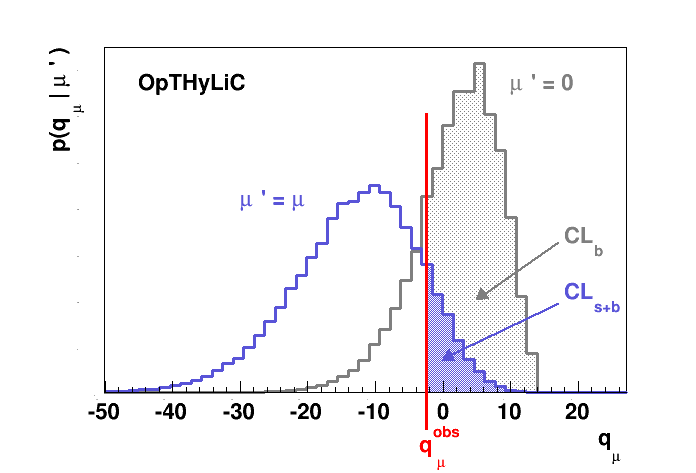
\includegraphics[scale=0.4]{figures/testStatDistribExample.png}
\caption{Exemple de distributions du test statistique sous l'hypoth\`ese signal plus bruit de fond ($\mu'=\mu$) et bruit de fond seul ($\mu'=0$). Les probabilit\'es \CLsb~et \CLb~sont repr\'esent\'ees par les aires color\'ees.\label{fig:testStatDistribExampleOTH}}
\end{center}
\end{figure}

\subsection{Traitement des incertitudes statistiques}
\label{sec:OTHTreatmentStatUncerts}

Les distributions \prior~des param\`etres de nuisance associ\'ees aux incertitudes statistiques sont de la forme (voir \'equation~\ref{eq:fullLhoodOTH})
\begin{equation}
\label{eq:statConstraintPdfGeneralForm}
f(y;y^{\text{nom}},\sigma)
\end{equation}
o\`u $y$ est le nombre d'\'ev\'enements attendu, $y^{\text{nom}}$ le nombre d'\'ev\'enements attendu nominal et $\sigma$ l'incertitude statistique (typiquement donn\'es par les \'equations~\ref{eq:yieldAndStatUncertFromWeights}). 
Les distributions disponibles sont gaussienne, log-normale et gamma (qui existe en trois d\'eclinaisons). 
%\begin{maliste}
%\item gaussienne
%\item log-normale 
%\item gamma (qui existe en trois d\'eclinaisons)
%\end{maliste}
Pour les distributions gaussienne et log-normale, les param\`etres sont choisis de telle sorte que l'esp\'erance et l'\'ecart-type soit \'egaux \`a $y^{\text{nom}}$ et $\sigma$ respectivement. 
La distribution gamma est justifi\'ee par le fait qu'il s'agit, pour un choix de distribution \prior~assez large, de la distribution \posterior~pour une exp\'erience auxiliaire poissonnienne\footnote{Nous ne consid\'erons dans ce qui suit que des distributions \prior~de la forme $y^\alpha$ mais c'est aussi le cas pour une distribution \prior~appartenant \`a la famille des distributions gamma.}. 
Dans la section~\ref{sec:statUncertTreatmentBayesian} nous avons vu que, pour une distribution \prior~de la forme $\pi\left(y\right)\propto y^\alpha$, la distribution \posterior~de $y$ est

\begin{equation}
\label{eq:gammaPriorsInOTH}
f\left(y;y^{\text{nom}},\sigma\right)=f_\text{G}\left(y;a=y^{\text{nom}}/\sigma^2,b=\left(y^{\text{nom}}/\sigma\right)^2+\alpha+1\right)
\end{equation}
o\`u $f_G\left(y;a,b\right)$ est la distribution gamma (\'equation~\ref{eq:gammaDistribution}). Dans \opthylic, les distributions gamma pour trois diff\'erentes valeurs de $\alpha$ ont \'et\'e choisies :
\begin{maliste}
\item $\pi\left(y\right)\propto 1$ ($\alpha=0$) : ce choix correspond \`a la distribution \prior~uniforme
\item $\pi\left(y\right)\propto 1/\sqrt{y}$ ($\alpha=-1/2$) : ce choix correspond \`a la distribution \prior~de Jeffreys
%, appr\'eci\'ee de beaucoup de bay\'esiens. 
%Rappelons que la distribution \prior~de Jeffrey est d'une mani\`ere g\'en\'erale donn\'ee par $\pi\left(y\right)\propto\sqrt{I(y)}$, o\`u l'information de Fisher est 
%\[I(y)=\E{\left(\frac{\dr\log P\left(N_\text{aux};y\right)}{\dr y}\right)^2}\] 
%$P\left(N_\text{aux};y\right)$ \'etant la fonction de vraisemblance de l'exp\'erience auxiliaire (voir section~\ref{sec:frequentistTreatmentOfStatUncert}) et qu'elle est invariante par reparam\'etrisation~\cite{Stuart:436225}.
\item $\pi\left(y\right)\propto 1/y$ ($\alpha=-1$) : ce choix est motiv\'e par le fait qu'il conduit \`a une distribution \posterior~de $y$ ayant pour esp\'erance $y^{\text{nom}}$ et pour \'ecart-type $\sigma$, comme dans le cas des distributions gaussienne et log-normale\footnote{L'esp\'erance et la variance de la distribution gamma de param\`etre d'intensit\'e $a$ et de forme $b$ sont $b/a$ et $b/a^2$ respectivement.}.
\end{maliste}

Notons que, pour les deux premiers choix de distribution \prior, ni l'esp\'erance ni l'\'ecart-type ne sont \'egaux \`a $y^{\text{nom}}$ et $\sigma$. Les cinq distributions disponibles dans \opthylic~sont compar\'ees sur la figure~\ref{fig:plotNormalLogNGamma} pour trois valeurs de $y^{\text{nom}}$ et $\sigma$. 

\begin{figure}[!htb]
\begin{center}
\hspace*{-0.5cm}
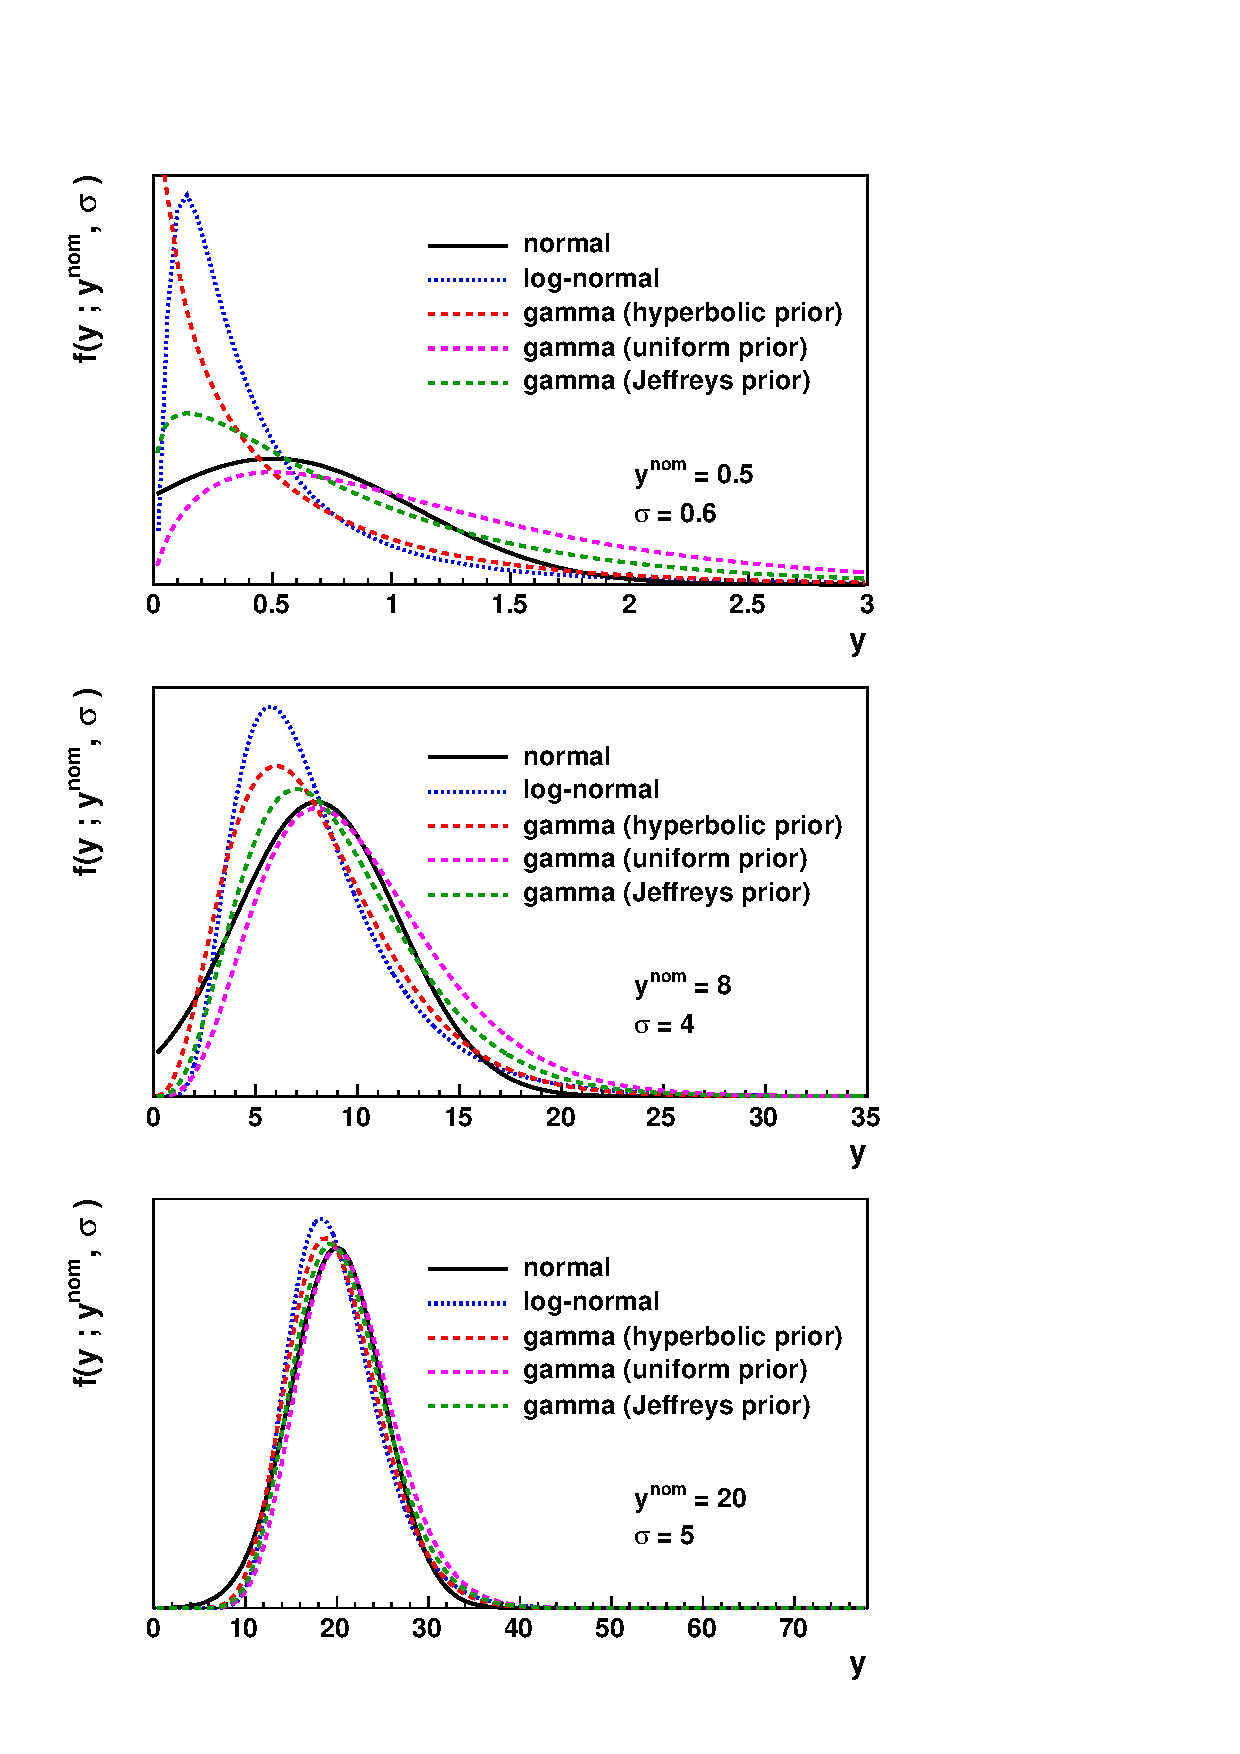
\includegraphics[width=0.5\textwidth]{figures/plotNormalLogNGamma.pdf}
\caption{Comparaison des densit\'es de probabilit\'es gaussienne, log-normale and gamma utilis\'ees comme distribution \prior~dans \opthylic~pour les incertitudes statistiques pour trois valeurs de $y^{\text{nom}}$ and $\sigma$.\label{fig:plotNormalLogNGamma}}
\end{center}
\end{figure}

\subsection{Traitement des incertitudes syst\'ematiques}
\label{sec:OTHTreatmentSystUncerts}

Les param\`etres de nuisance associ\'es aux incertitudes syst\'ematiques (les $\eta_j$ dans les \'equations~\ref{eq:sigYieldOTH}, \ref{eq:bkgYieldOTH} et \ref{eq:fullLhoodOTH}) sont choisis de telle sorte que la valeur nominale soit \'egale \`a 0 et que les valeurs correspondant \`a des variations de $\pm 1\sigma$ des sources d'incertitudes soient \'egales \`a $\pm 1$. 
Un tel choix permet d'avoir un traitement unifi\'e de toutes les incertitudes syst\'ematiques consid\'er\'ees. 
Notons $y^\text{var}_j$ et $\fsyst_j\left(\eta_j\right)$ le nombre d'\'ev\'enements vari\'es et le rapport entre ce nombre et le nombre nominal pour l'incertitude $j$ respectivement :
\begin{equation}
\label{eq:yvarVSynomANDsystevariation}
y^\text{var}_j=y^\text{nom}\times \fsyst_j\left(\eta_j\right)
\end{equation}

%Nous avons par construction
%\[\fsyst_j\left(\eta_j=0\right)=1\]
%et, en notant $\ffup_j$ et $\ffdown_j$ les incertitudes relatives sur les nombres d'\'ev\'enements pour l'incertitude $j$,
%\begin{subequations} 
%\label{eq:systFuncConstraint}
%  \begin{gather}
%    \ffup_j=\fsyst_j\left(\eta_j=+1\right)-1 \label{eq:systFuncConstraint2} \\
%    \ffdown_j=\fsyst_j\left(\eta_j=-1\right)-1 \label{eq:systFuncConstraint3}
%  \end{gather}
%\end{subequations}

%Comme il a \'et\'e dit pr\'ec\'edemment, une limitation dans le traitement des incertitudes syst\'ematiques provient du fait que seuls $\fsyst_j\left(\eta_j\right)$ pour $\eta_j=0, -1$ et $+1$ 
%(et donc $\ffup_j$ et $\ffdown_j$) 
%sont connus. 
Pour chacune incertitude syst\'ematique, \opthylic~utilise uniquement les valeurs des nombres d'\'ev\'enements vari\'es lorsque les sources d'incertitudes sont vari\'ees de $\pm 1\sigma$. 
Ainsi, seules les valeurs de $\fsyst_j\left(\eta_j\right)$ pour $\eta_j=0, -1$ et $+1$ sont connues (celle pour $\eta_j=0$ valant 1 par construction).
Pour d\'eterminer $\fsyst_j\left(\eta_j\right)$ pour d'autres valeurs de $\eta_j$, il est n\'ecessaire d'interpoler entre $-1$ et $+1$ et d'extrapoler au-del\`a. Les contraintes imposées \`a ces fonctions d'interpolation et d'extrapolation sont premi\`erement qu'elles doivent passer, au moins approximativement, par les valeurs mesurées expérimentalement et deuxièmement qu'elles doivent être monotones. Gr\^ace \`a cette derni\`ere condition les intervalles $\eta_j\in\left[-1;+1\right]$ et $y^\text{var}_j\left(\eta_j\right)\in\left[y^\text{var}_j\left(\eta_j=-1\right);y^\text{var}_j\left(\eta_j=+1\right)\right]$ correspondent \`a un m\^eme niveau de confiance ou de crédibilité (68,3\% dans notre cas). 

Quatre choix de fonctions d'interpolation et d'extrapolation sont disponibles dans \opthylic{} : interpolation et extrapolation lin\'eaire par partie, interpolation et extrapolation exponentielle par partie, interpolation polynomiale et extrapolation exponentielle, interpolation et extrapolation similaire \`a celle disponible dans le programme \mclimit.
%Les choix disponibles dans \opthylic{} sont :
%\begin{maliste}
%\item interpolation et extrapolation lin\'eaire par partie
%\item interpolation et extrapolation exponentielle par partie
%\item interpolation polynomiale et extrapolation exponentielle
%\item interpolation et extrapolation similaire \`a celle disponible dans le programme \mclimit.
%\end{maliste}
Ces diff\'erents choix sont repr\'esent\'es sur la figure~\ref{fig:ExampleFunctionsInterExtrap} pour diff\'erentes valeurs de 
%$\ffup_j$ et $\ffdown_j$.
$\fsyst_j\left(\eta_j=-1\right)$ et $\fsyst_j\left(\eta_j=+1\right)$.
\vspace{-0.2cm}
\enlargethispage{2.5cm}
\begin{figure}[!htb]
\begin{center}
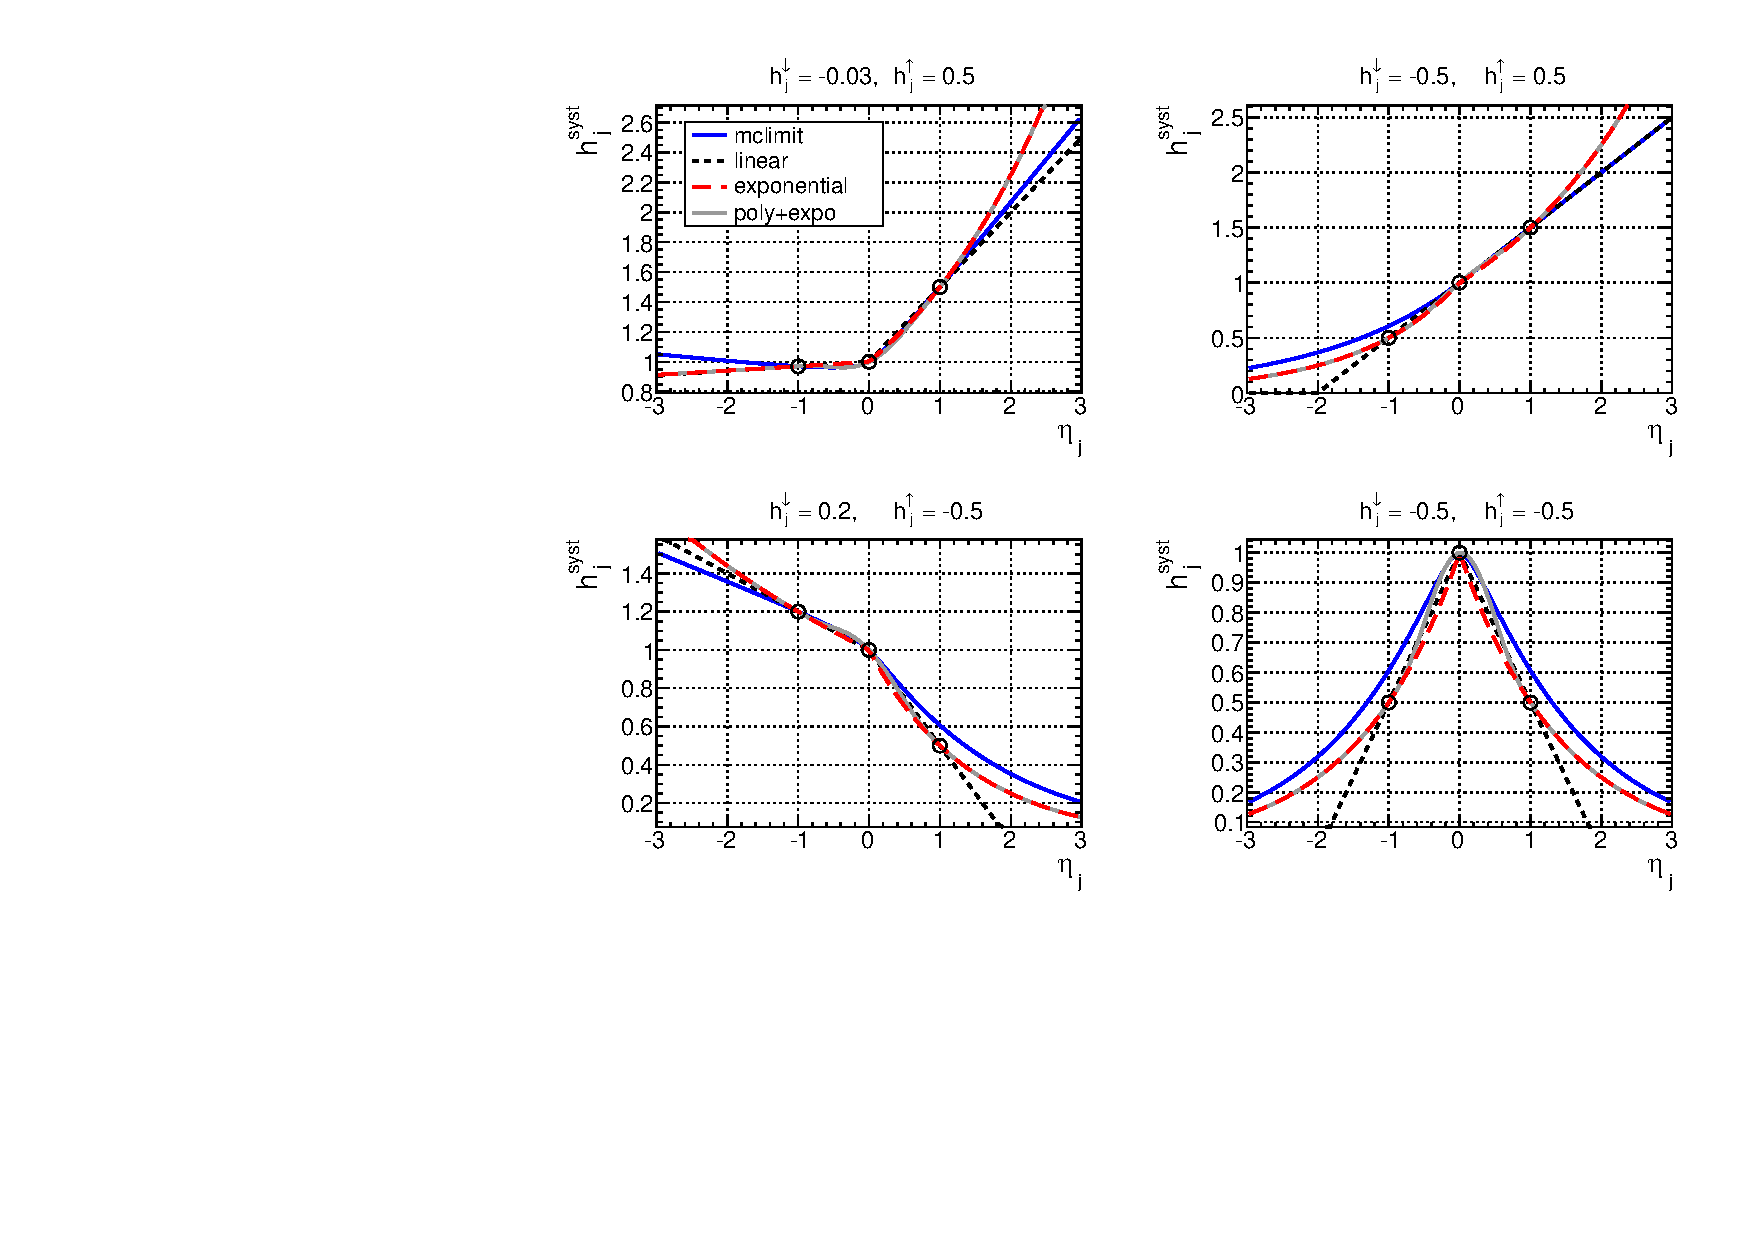
\includegraphics[scale=0.7]{figures/cFunctionsInterExtrap.pdf}
\caption{Illustration des interpolations et extrapolations disponibles dans \opthylic~pour diff\'erentes valeurs de $\fsyst_j\left(\eta_j=-1\right)$ et $\fsyst_j\left(\eta_j=+1\right)$. Les grandeurs $\ffdown_j$ et $\ffup_j$ dont les valeurs sont donn\'ees sur chaque graphique correspondent aux variations relatives sur les nombres d'\'ev\'enements lorsque la source d'incertitude est vari\'ee de $-1\sigma$ et $+1\sigma$ respectivement.
%$\ffdown_j=-0.03$ et $\ffup_j=0.5$, $\ffdown_j=-0.5$ et $\ffup_j=0.5$, $\ffdown_j=0.5$ et $\ffup_j=0.5$ et $\ffdown_j=-0.5$ et $\ffup_j=-0.5$.
\label{fig:ExampleFunctionsInterExtrap}}
\end{center}
\end{figure}

%\vspace{-0.7cm}
Comme le montre cette figure, 
%le choix similaire \`a celui du programme \mclimit~pr\'esente la particularit\'e de ne v\'erifier les \'equations~\ref{eq:systFuncConstraint} qu'approximativement lorsque $\ffup_j$ et $\ffdown_j$ sont n\'egatifs. 
la fonction d'interpolation et d'extrapolation utilis\'ee par le programme \mclimit{} ne v\'erifie l'equation~\ref{eq:yvarVSynomANDsystevariation} qu'approximativement lorsque $\fsyst_j\left(\eta_j=-1\right)$ ou $\fsyst_j\left(\eta_j=+1\right)$ est inf\'erieur \`a 1.
Ceci peut \^etre per\c cu comme ind\'esirable. Ce choix est malgr\'e tout disponible dans \opthylic~pour permettre des comparaisons avec \mclimit. De telles comparaisons ont par exemple \'et\'e effectu\'ees pour valider \opthylic~(voir section~\ref{sec:validationOTH}).

%Rappelons encore une fois que 
Comme il a \'et\'e dit pr\'ec\'edemment, le choix de l'interpolation et de l'extrapolation est dans une grande mesure arbitraire. Il est tr\`es probable qu'aucun des choix pr\'esent\'es ci-dessus ne corresponde \`a la r\'ealit\'e. D'o\`u l'importance d'\'etudier la stabilit\'e des r\'esultats avec ces choix. Une solution (ou du moins une am\'elioration) serait de mesurer les nombres d'événements variés pour plus de variations dans les sources d'incertitudes (c'est-\`a-dire d'ajouter par exemple les variations pour $\pm 2\sigma,\pm 3\sigma,\hdots$). Ceci serait extr\^emement lourd \`a mettre en place en pratique et n'est, pour cette raison, pas fait en physique des particules pour l'instant\footnote{Il s'agit ici non pas d'une limitation li\'ee \`a la prise en compte de ces variations suppl\'ementaires au sein d'un programme de calcul de limite mais d'une limitation li\'ee au temps n\'ecessaire pour calculer les nombres d'\'ev\'enements vari\'es.}.

\subsection{Limites attendues sous l'hypoth\`ese de bruit de fond}
\label{sec:limitesAttenduesHypBdf}

En plus des limites d'exclusion observ\'ees, \opthylic~permet de calculer les limites d'exclusion attendues sous l'hypoth\`ese de bruit de fond m\'ediane et \`a $-2\sigma$, $-1\sigma$, $+1\sigma$ et $+2\sigma$. Ceci peut \^etre fait par deux méthodes. Dans la premi\`ere, la distribution de la limite observ\'ee sous l'hypoth\`ese de bruit de fond est d\'etermin\'ee. Les cinq limites attendues sont obtenues en d\'eterminant les quantiles de cette distribution. Dans la deuxi\`eme, les limites attendues sont calcul\'ees comme la limite observ\'ee mais en repla\c cant le \CLs~observ\'e par les quantiles de la distribution de \CLs~sous l'hypoth\`ese de bruit de fond.

Les deux m\'ethodes sont \'equivalentes.
% du point de vue statistique. 
Pour le prouver, explicitons la dépendance en $\qmuobs$ de \CLs. La limite supérieure observée $\mup$ est donc donnée par
\begin{equation}
\label{eq:CLsDefUpperLimitqmuobsExplicited}
\CLs\left(\mup,\qmuobs\right)=\alpha
\end{equation}

La première méthode consiste à calculer les quantiles de la distribution de $\mup$ sous l'hypothèse de bruit de fond. \`A partir de l'expression précédente, nous pouvons écrire 
\[\mup=\CLs^{-1}\left(\alpha,\qmuobs\right)\]
où $\CLs^{-1}$ est la fonction inverse de \CLs. Les quantiles de $\mup$ sont donc (en notant $\text{quant}_p\left[X\right]$ le quantile $p$ de la variable aléatoire $X$)
\begin{equation}
\label{eq:quantileDefFirstMethod}
\text{quant}_p\left[\mup\right]=\text{quant}_p\left[\CLs^{-1}\left(\alpha,\qmuobs\right)\right]
\end{equation}

La deuxième méthode consiste à résoudre l'équation~\ref{eq:CLsDefUpperLimitqmuobsExplicited} en utilisant les quantiles de la distribution de \CLs. Soit $\mup^p$ la solution de cette équation pour le quantile $p$. Nous avons
\[\text{quant}_p\left[\CLs\left(\mup^p,\qmuobs\right)\right]=\alpha\] 

Or, dans tous les cas que nous avons examin\'e en pratique, $\CLs$ est une fonction monotone de $\qmuobs$, donc
\[\CLs\left(\mup^p,\text{quant}_p\left[\qmuobs\right]\right)=\alpha\] 
soit
\begin{equation}
\label{eq:quantileDefSecondMethod}
\mup^p=\CLs^{-1}\left(\alpha,\text{quant}_p\left[\qmuobs\right]\right)=\text{quant}_p\left[\CLs^{-1}\left(\alpha,\qmuobs\right)\right]
\end{equation}

Des équations \ref{eq:quantileDefFirstMethod} et \ref{eq:quantileDefSecondMethod} nous déduisons que $\mup^p=\text{quant}_p\left[\mup\right]$, ce qui prouve l'équivalence des deux méthodes. Elles sont en revanche tr\`es diff\'erentes en terme de temps de calcul. Pour la premi\`ere, de nouvelles pseudo-exp\'eriences doivent \^etre faites pour d\'eterminer la distribution de $\mup$ en plus des pseudo-exp\'eriences d\'ej\`a r\'ealis\'ees pour d\'eterminer les distributions du test statistique pour chaque valeur de $\mu$. Pour la deuxi\`eme, ces derni\`eres pseudo-exp\'eriences peuvent \^etre r\'eutilis\'ees pour d\'eterminer la distribution puis les quantiles de \CLs. La deuxi\`eme m\'ethode est de ce fait beaucoup plus rapide que la premi\`ere, notamment lorsque le nombre de canaux est \'elev\'e. Seuls les r\'esultats obtenus avec la deuxi\`eme m\'ethode seront pr\'esent\'es dans la suite de ce document.

\section{Approche bayésienne : \tifosi} 
\label{sec:tifosi}

En parall\`ele d'\opthylic, un outil impl\'ementant l'approche bay\'esienne a \'et\'e d\'evelopp\'e. 
Cet outil, nomm\'e \tifosi~(ToolkIt FOr Statistical Interpretation), a \'et\'e utilis\'e pour calculer les limites d'exclusion dans les analyses d\'ecrites dans le chapitre~\ref{chap:Recherche4tops} suivant une m\'ethode purement bay\'esienne, afin de les comparer \`a celles obtenues par \mclimit~et \opthylic.
%Il a aussi \'et\'e utilis\'e pour valider les calculs r\'ealis\'es par \opthylic, notamment le traitement des incertitudes statistiques et syst\'ematiques, gr\^ace au r\'esultat pr\'esent\'e dans la section~\ref{eq:equivalenceHybridBayesian}. 


%dans deux objectifs. 
%Le premier est la validation des calculs r\'ealis\'es par \opthylic, notamment le traitement des incertitudes statistiques et syst\'ematiques. 
%En effet, comme nous l'avons vu dans la section~\ref{eq:equivalenceHybridBayesian}, les approches hybride et bay\'esienne sont \'equivalentes sous certaines conditions. 
%Comparer les limites d'exclusion calcul\'ees par \tifosi~\`a celles calcul\'ees par \opthylic~permet par cons\'equent de valider ce dernier outil. 
%Le deuxi\`eme est le calcul des limites finales des analyses d\'ecrites dans le chapitre~\ref{chap:Recherche4tops} suivant une m\'ethode purement bay\'esienne, afin de les comparer \`a celles obtenues par \mclimit~et \opthylic.

\subsection{Description}

\tifosi~est un outil bas\'e sur \roofit~et \roostats. Le mod\`ele statistique (c'est-\`a-dire la fonction de vraisemblance, les distributions \prior~et les interpolations/extrapolations) a \'et\'e impl\'ement\'e avec \roofit~et l'inf\'erence bay\'esienne est r\'ealis\'ee avec \roostats. 

Afin de pouvoir permettre des comparaisons directe avec \opthylic, le mod\`ele statistique implement\'e dans \tifosi~est le m\^eme que celui impl\'ement\'e dans \opthylic. La fonction de vraisemblance est donn\'ee dans l'\'equation~\ref{eq:fullLhoodOTH}. Les distributions \prior~pour les incertitudes statistiques et syst\'ematiques sont les m\^emes que celles d\'ecrites dans les sections~\ref{sec:OTHTreatmentStatUncerts} et \ref{sec:OTHTreatmentSystUncerts}. Les interpolations et extrapolations sont r\'ealis\'ees avec le m\^eme code que celui utilis\'e dans l'outil \histfactory~\cite{Cranmer:1456844}. Il est possible de r\'ealiser, comme dans \opthylic, des interpolations et extrapolations lin\'eaires, exponentielles et polynomiales+exponentielles. L'interpolation et extrapolation du programme \mclimit~n'est en revanche pas disponible.

La d\'etermination de la distribution \posterior~conjointe (\'equation~\ref{eq:jointPosteriorPIandNuisance}) est r\'ealis\'ee avec \roostats~par m\'ethode Monte Carlo avec cha\^ine de Markov. L'algorithme utilis\'e est d\'ecrit dans la section suivante.

\tifosi~est
%, comme \opthylic,
 un outil d\'edi\'e au calcul de limites d'exclusion pour les exp\'eriences de comptage. Le nombre de canaux est arbitraire, ainsi que le nombre de sources de bruit de fond et d'incertitudes syst\'ematiques. Le format de fichier d'entr\'ee dans \tifosi~est le m\^eme que celui dans \opthylic, ce qui permet des comparaisons directes.

\subsection{Algorithme de Metropolis-Hastings}
\label{sec:MCMC}

L'inf\'erence bay\'esienne passe par la d\'etermination de la distribution \posterior~conjointe des param\`etres d'int\'er\^et et de nuisance. Nous avons utilis\'e pour cela une m\'ethode Monte Carlo par cha\^ine de Markov utilisant l'algorithme de Metropolis-Hastings~\cite{Stuart:436225,delemontex:in2p3-00844359}. 
%Cet algorithme est d\'ecrit bri\`evement ci-dessous.
Cet algorithme,
particuli\`erement bien adapt\'e pour les probl\`emes \`a grand nombre de dimensions comme le notre, 
permet d'\'echantillonner n'importe quelle densit\'e de probabilit\'e.
%, dans notre cas la distribution \posterior~conjointe dans l'\'equation~\ref{eq:jointPosteriorPIandNuisance}. 
La densit\'e de probabilit\'e calcul\'ee \`a partir de l'\'echantillon converge vers la densit\'e souhait\'ee lorsque le nombre d'\'el\'ements dans la cha\^ine tend vers l'infini. 

Afin de simplifier la description qui suit, nous noterons la distribution \posterior~conjointe $\Lh\left(\theta\right)$ ($\theta$ d\'esigne l'ensemble form\'e du param\`etre d'int\'er\^et et des param\`etres de nuisance). Les \'el\'ements de la cha\^ine de Markov, not\'es $\theta_i$, sont trouv\'es de la mani\`ere suivante. \`A chaque it\'eration $i$, un nouveau point dans l'espace des param\`etres $\theta^\star$ est propos\'e suivant une "loi de proposition" $q\left(\theta^\star|\theta_i\right)$. L'acceptation de ce nouveau point est bas\'ee sur la grandeur
\[\rho=\text{min}\left(1,\frac{\Lh\left(\theta^\star\right)}{\Lh\left(\theta_i\right)}\frac{q\left(\theta_i|\theta^\star\right)}{q\left(\theta^\star|\theta_i\right)}\right)\]
 
$\rho$ est compar\'e \`a un nombre $u$ tir\'e al\'eatoirement suivant une loi uniforme entre $0$ et $1$. Si $u<\rho$, $\theta^\star$ est accept\'e. Sinon il est rejet\'e et un nouveau point est propos\'e \`a partir de $\theta_i$.

La loi de proposition utilis\'ee ici est une loi multinormale avec une matrice de covariance fixe. Cette loi \'etant sym\'etrique, nous avons $q\left(\theta_i|\theta^\star\right)=q\left(\theta^\star|\theta_i\right)$. Ainsi $\rho$ se simplifie en
\[\rho=\text{min}\left(1,\frac{\Lh\left(\theta^\star\right)}{\Lh\left(\theta_i\right)}\right)\]

Afin d'illustrer cet algorithme, nous avons consid\'er\'e le cas simple d'un seul canal avec un nombre d'\'ev\'enements de signal attendu nominal parfaitement connu ($s=1$) et un unique bruit de fond entach\'e d'une incertitude statistique ($b=10\pm3$) contraint par une distribution \prior~gaussienne. Le nombre d'\'ev\'enements observ\'es est $10$. La figure~\ref{fig:Posterior2DPoissonWithUncertainBkg} montre la distribution \posterior~conjointe de $b$ et $\mu$ (\`a gauche) et la distribution \posterior~de $\mu$ apr\`es marginalisation sur le param\`etre de nuisance (\`a droite). Ces deux distributions ont \'et\'e obtenues avec un total de $10^7$ iterations dans la cha\^ine de Markov. 

\begin{figure}[!htb]
\begin{center}
\hspace*{-0.6cm}
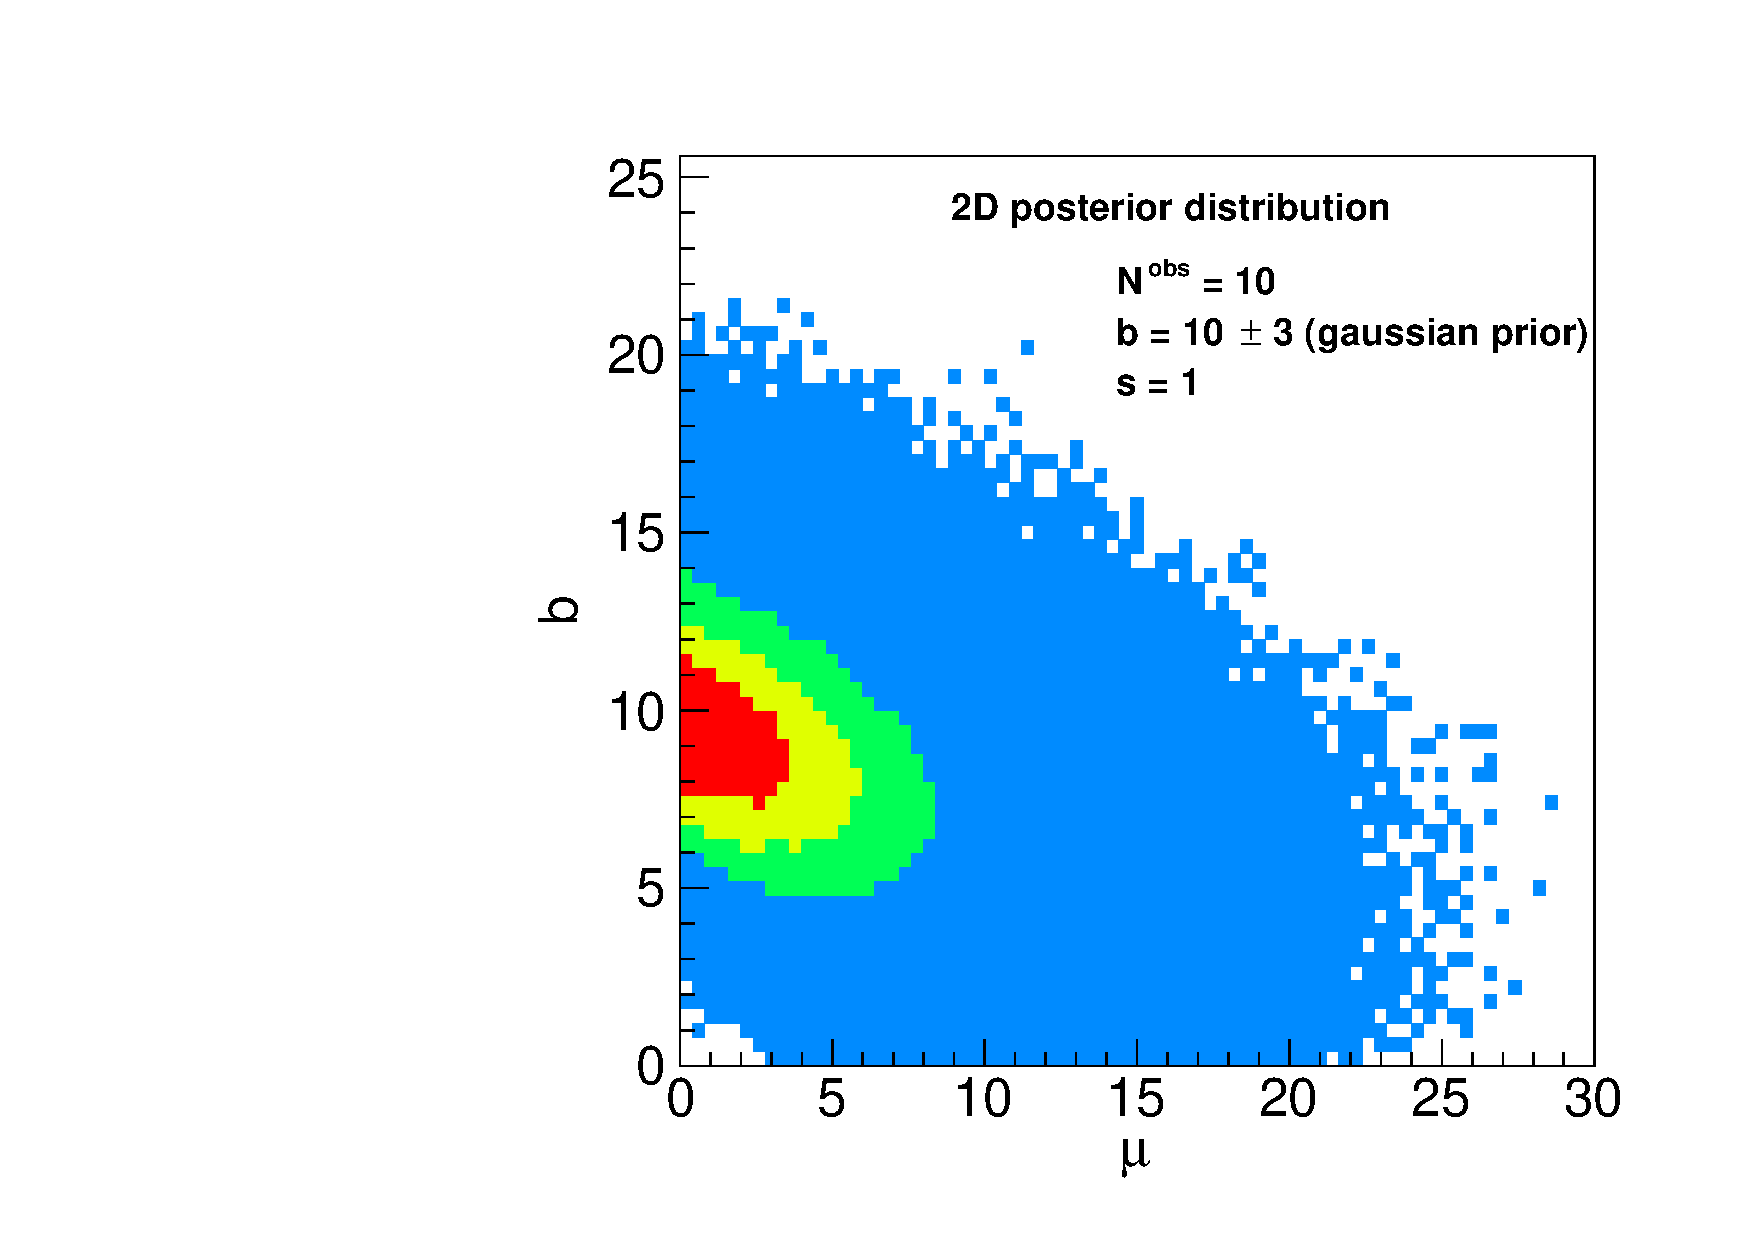
\includegraphics[scale=0.35]{figures/Posterior2DPoissonWithUncertainBkg.pdf}
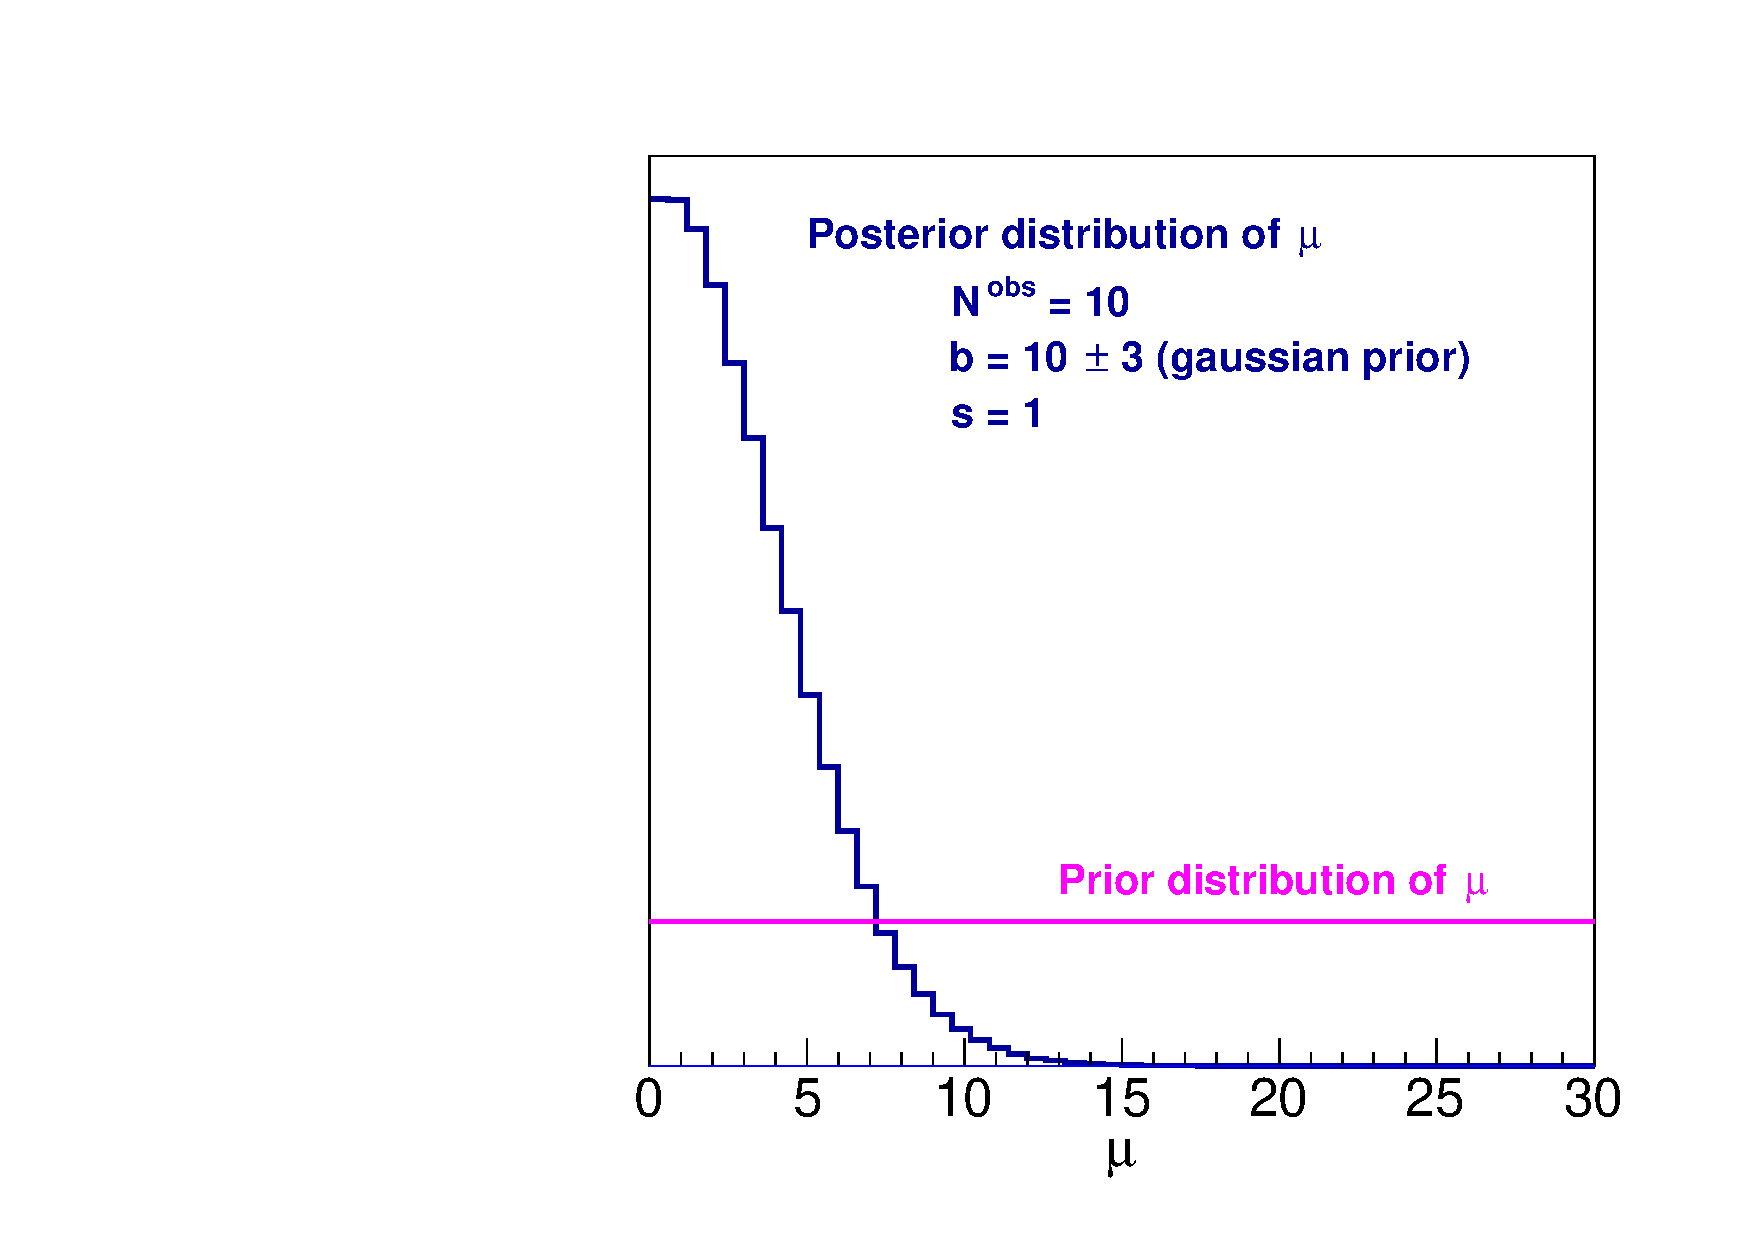
\includegraphics[scale=0.35]{figures/PosteriorSignalPoissonWithUncertainBkg.pdf}
\caption{Exemples de distribution \posterior~\`a 2 dimensions (\`a gauche) et de distribution \posterior~sur le param\`etre d'int\'er\^et $\mu$ (\`a droite).\label{fig:Posterior2DPoissonWithUncertainBkg}}
\end{center}
\end{figure}

La figure~\ref{fig:illustrationConvergeMarkovChainMu} 
%(\ref{fig:illustrationConvergeMarkovChainBkg}) 
montre la valeur moyenne et l'\'ecart-type de la distribution \posterior~de $\mu$ 
%($b$) 
apr\`es chaque itération pour laquelle le point propos\'e $\theta^\star$ est accept\'e (le taux d'acceptation est ici d'environ 18\%). Le nombre total d'it\'erations est de $10^5$. La cha\^ine converge apr\`es environ $1000$~iterations accept\'ees, soit environ $5000$~iterations totales. Les distributions pr\'esent\'ees sur la figure~\ref{fig:Posterior2DPoissonWithUncertainBkg} et calcul\'ees avec un total de $10^7$ iterations sont donc des estimations fiables des distributions \posterior.
 
\begin{figure}[!htb]
\begin{center}
\hspace*{-0.6cm}
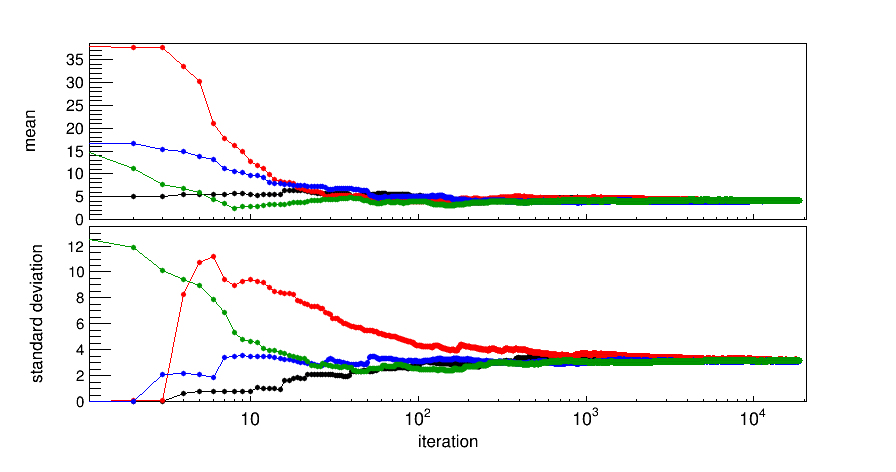
\includegraphics[scale=0.45]{macros/cMu.png}
\caption{Valeur moyenne et \'ecart-type de la distribution \posterior~du param\`etre d'int\'er\^et $\mu$ en fonction du nombre d'it\'erations pour l'exemple d\'ecrit dans le texte et pour différentes points de départ de la cha\^ine de Markov.\label{fig:illustrationConvergeMarkovChainMu}}
\end{center}
\end{figure}

%\begin{figure}[!htb]
%\begin{center}
%\hspace*{-0.6cm}
%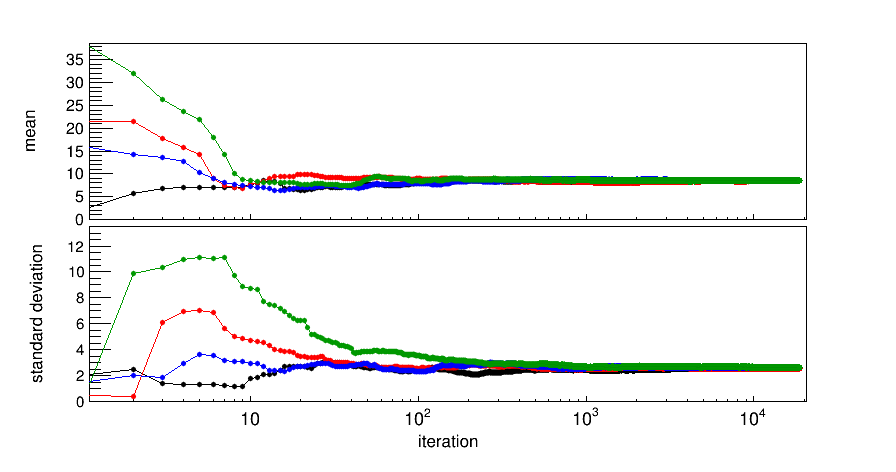
\includegraphics[scale=0.45]{macros/cBkg.png}
%\caption{Valeur moyenne et \'ecart-type de la distribution \posterior~du nombre de bruit de fond attendu $b$ en fonction du nombre d'it\'erations pour l'exemple d\'ecrit dans le texte et pour différentes points de départ de la cha\^ine de Markov.\label{fig:illustrationConvergeMarkovChainBkg}}
%\end{center}
%\end{figure}

%\section{Conclusion}

%Les outils \opthylic~et \tifosi~impl\'ement\'es pour le calcul de limite 
%d'exclusion sur les sections efficaces de production ont \'et\'e 
%pr\'esent\'es. Ces outils utilisent le m\^eme mod\`ele statistique et sont 
%capables de prendre en compte un nombre arbitrairement grand d'incertitudes 
%statistiques et syst\'ematiques. Les corr\'elations entre ces derni\`eres sont 
%\'egalement prises en compte. Les calculs r\'ealis\'es par ces outils sont 
%souvent non triviaux. Ils doivent par cons\'equent \^etre valid\'es avant de 
%pouvoir \^etre utilis\'es dans une analyse de physique. Le chapitre suivant 
%pr\'esente les \'etudes r\'ealis\'ees pour valider \opthylic.

%\chapter{Validation d'\opthylic} 
\section{Validation} 
\label{sec:validationOTH} 

La d\'etermination des limites d'exclusion 
%(observ\'ees et attendues) 
avec \opthylic~et \tifosi~implique de nombreux calculs de diff\'erents types : g\'en\'eration 
de nombres al\'eatoires, calcul de \pval s, it\'eration sur 
les valeurs de $\mu$ pour r\'esoudre l'\'equation~\ref{eq:hybrideCLSLimitDef}, 
combinaison des canaux, interpolation et extrapolation pour les incertitudes 
syst\'ematiques, \'evaluation et marginalisation de la fonction de vraisemblance, calcul de quantiles, etc. 
De nombreuses \'etudes ont \'et\'e r\'ealis\'ees pour valider ces calculs. \opthylic~et \tifosi~ont \'et\'e 
%est compar\'e 
compar\'es soit \`a des solutions th\'eoriques lorsque cela est possible, soit entre eux
lorsque les calculs hybrides et bay\'esiens sont \'equivalents.
\opthylic~a \'egalement \'et\'e compar\'e au programme \mclimit~qui est \'equivalent \`a \opthylic~lorsque les bons choix sont faits pour l'interpolation et l'extrapolation et pour les distributions \prior. 
Ces \'etudes sont d\'ecrites dans cette section.

%\section{Calcul sur un canal sans incertitudes}
%\subsection{Calcul sur un canal sans incertitudes}
\subsection{Validation des calculs en l'absence d'incertitudes}

\opthylic~
%a d'abord \'et\'e valid\'e 
et \tifosi~ont d'abord \'et\'e valid\'es dans la situation la plus simple o\`u le nombre d'\'ev\'enements de signal et le bruit de fond attendu est parfaitement connu. 
Lorsqu'il y a un seul canal, les approches hybride et bay\'esienne sont \'equivalentes et il existe une solution analytique pour \mup~\cite{Busato:2015ola} :
%. 
%En effet, \CLsb~et \CLb~sont donn\'es par
%\[\CLsb=\sum\limits_{\n=0}^{\nobs}\frac{\left(\mu\snom+\bnom\right)^{\n}}{\n!} e^{-\left(\mu\snom+\bnom\right)}=1-F_{\chi^2}\left(2\left(\mu\snom+\bnom\right);2\left(\nobs+1\right)\right)\]
%et
%\[\CLb=\sum\limits_{\n=0}^{\nobs}\frac{\left(\bnom\right)^{\n}}{\n!} e^{-\bnom}=1-F_{\chi^2}\left(2\bnom;2\left(\nobs+1\right)\right)\]
%o\`u $F_{\chi^2}\left(x;d\right)$ est la valeur de la fonction de repartition de la loi de chi-carr\'e avec $d$ degr\'es de libert\'es en $x$. L'\'equation \ref{eq:CLsDefOfMup} conduit donc \`a 
\begin{equation}
\label{eq:muUpAnalyticalResultWoUncert}
\mup=\frac{0.5\times F_{\chi^{2}}^{-1}\left(1-\alpha\left[1-F_{\chi^{2}}\left(2\bnom;2\left(\nobs+1\right)\right)\right];2\left(\nobs+1\right)\right)-\bnom}{\snom}
\end{equation}
o\`u $F_{\chi^2}\left(x;d\right)$ est la fonction de repartition de la loi de chi-carr\'e avec $d$ degr\'es de libert\'es en $x$. 
La figure \ref{fig:ExampleValidNoUncertVsAnalytical} montre une comparaison entre cette solution analytique et \opthylic~pour $\bnom=0.82\times L$, $\snom=2.49\times L$ et $\nobs=1\times L$, avec $L=1,\hdots,7$. 
L'accord entre les deux est excellent. 
D'autres tests ont \'et\'e r\'ealis\'es avec des valeurs diff\'erentes de $\bnom$, $\snom$ et $\nobs$. 
Tous montrent un accord de la m\^eme qualit\'e.
Des comparaisons similaires ont \'et\'e faites entre l'\'equation~\ref{eq:muUpAnalyticalResultWoUncert} et \tifosi. 
\`A chaque fois, un tr\`es bon accord a \'et\'e obtenu.

\begin{figure}[!htb]
\begin{center}
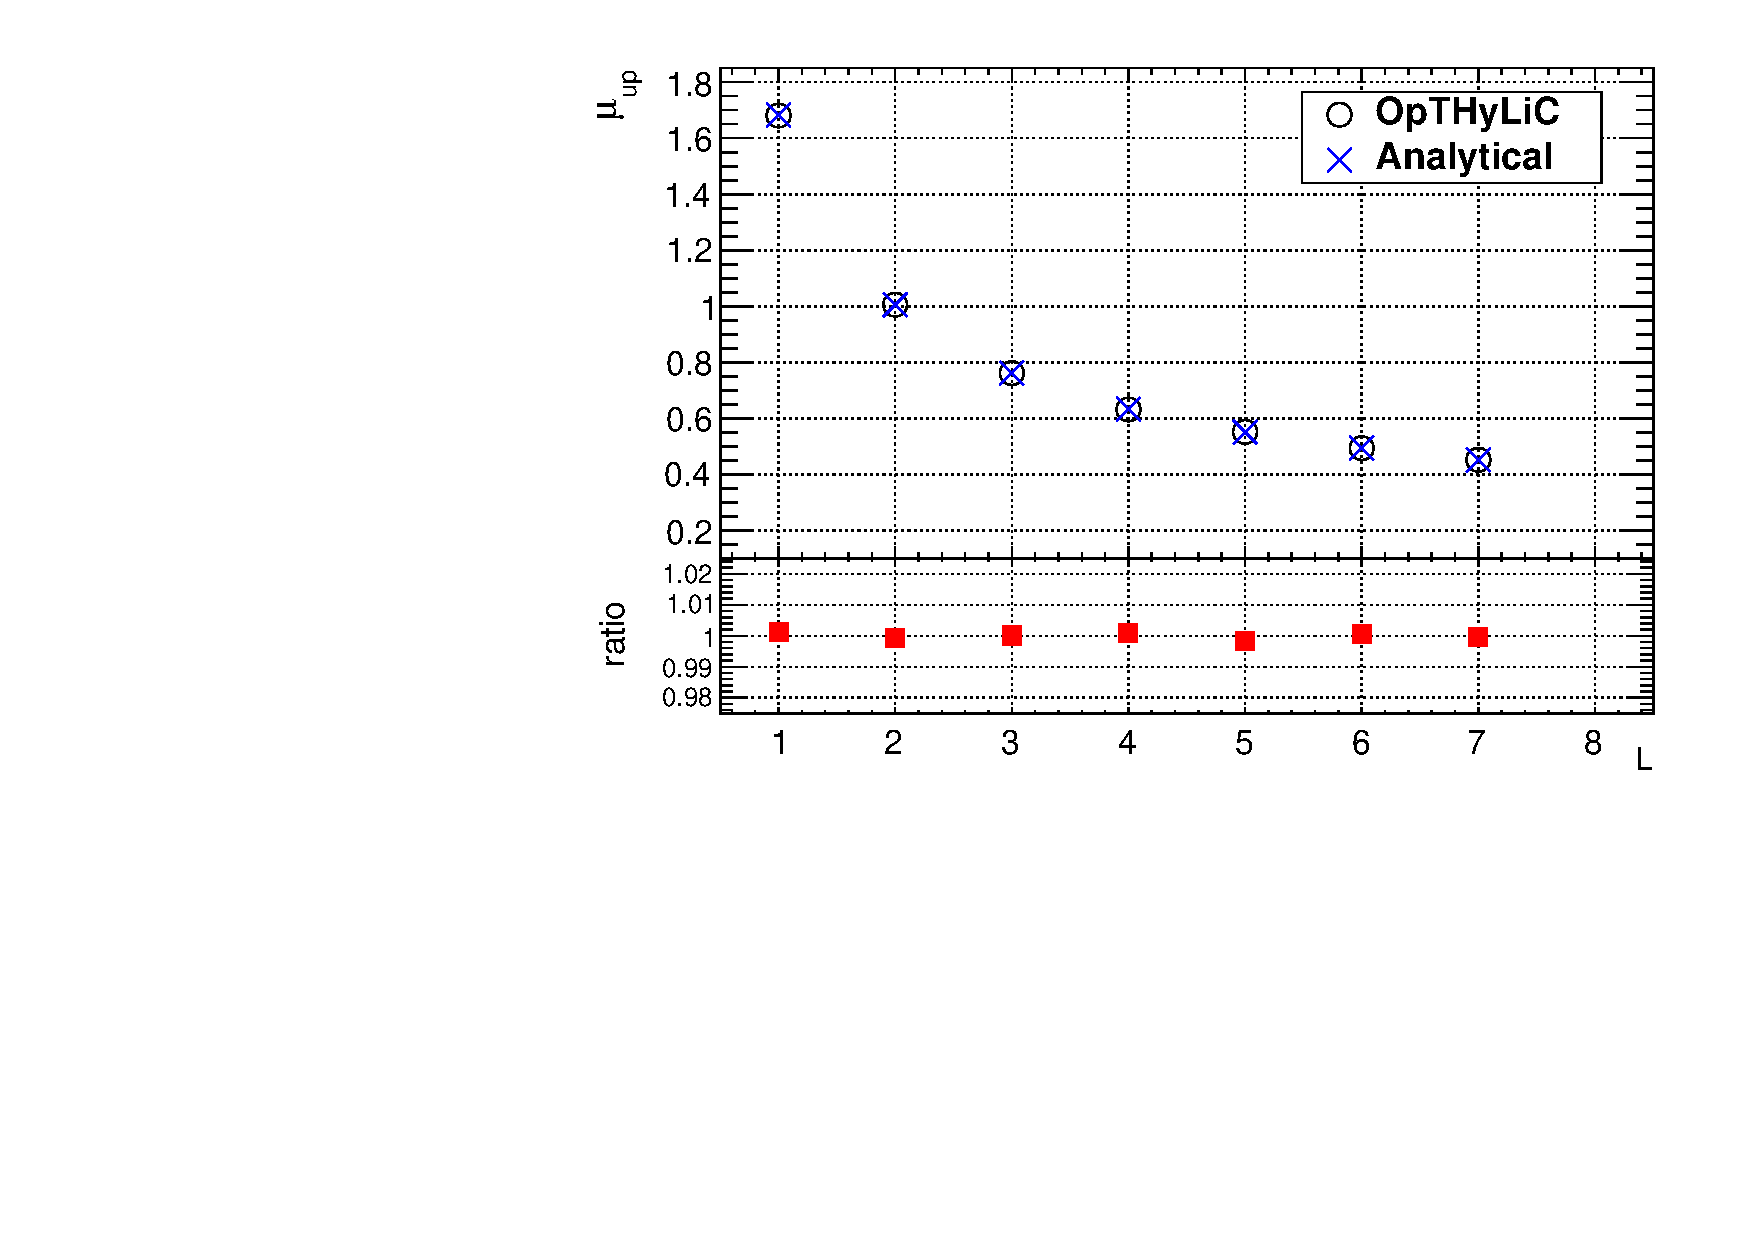
\includegraphics[scale=0.5]{figures/SingleChannelNoUncertainties.pdf}
\caption{Limite d'exclusion en fonction de $L$ calcul\'ee avec \opthylic~et \`a partir du r\'esultat analytique (\'equation~\ref{eq:muUpAnalyticalResultWoUncert}) pour $\bnom=0.82\times L$, $\snom=2.49\times L$ et $\nobs=1\times L$.\label{fig:ExampleValidNoUncertVsAnalytical}}
\end{center}
\end{figure}

%\section{Calcul sur plusieurs canaux sans incertitudes}
%\subsection{Calcul sur plusieurs canaux sans incertitudes}

Dans le cas o\`u plusieurs canaux d'analyse sont combin\'es, deux validations ont \'et\'e faites. Premi\`erement, les limites d'exclusion obtenues avec plusieurs canaux sont compar\'ees aux limites d'exclusion obtenues avec un seul canal dans des situations o\`u les deux doivent donner des r\'esultats identiques. De telles situations se produisent lorsque les nombres d'\'ev\'enements dans les diff\'erents canaux sont reli\'es les uns aux autres par un facteur multiplicatif. Par exemple, les m\^emes limites doivent \^etre trouv\'ees dans les deux cas suivants :
\begin{maliste}
\item \nochan~canaux avec $\bnom/\nochan$ \'ev\'enements de bruit de fond, $\snom/\nochan$ \'ev\'enements de signal et $\nobs/\nochan$ \'ev\'enements observ\'es
%\begin{itemize}
%\item nombre d'\'ev\'enements de bruit de fond=$\bnom/\nochan$
%\item nombre d'\'ev\'enements de signal=$\snom/\nochan$
%\item nombre d'\'ev\'enements observ\'es=$\nobs/\nochan$
%\end{itemize}
\item un canal avec $\bnom$ \'ev\'enements de bruit de fond, $\snom$ \'ev\'enements de signal et $\nobs$ \'ev\'enements observ\'es

%\begin{itemize}
%\item nombre d'\'ev\'enements de bruit de fond=$\bnom$
%\item nombre d'\'ev\'enements de signal=$\snom$
%\item nombre d'\'ev\'enements observ\'es=$\nobs$
%\end{itemize}
\end{maliste}

Les calculs dans ces deux cas ont \'et\'e compar\'es pour plusieurs valeurs de \snom, \bnom, \nobs~et \nochan. \opthylic~et \tifosi~trouvent, comme il se doit, les m\^emes limites d'exclusion. Deuxi\`emement, nous avons consid\'er\'e le cas g\'en\'eral o\`u les nombres d'\'ev\'enements dans les diff\'erents canaux ne peuvent pas \^etre reli\'es entre eux par un facteur multiplicatif. D'apr\`es les \'equations \ref{eq:testStatOTHAllChannels} et \ref{eq:testStatOTHChannelc} nous voyons que le test statistique utilis\'e dans \opthylic{} peut s'\'ecrire
\[\n_{\text{eff}}=\sum\limits_c \nc\beta_c\quad\text{avec}\quad\beta_c=\ln\frac{\mu\scnom+\sum\limits_i\bcinom}{\sum\limits_i\bcinom}\] 

Dans la limite asymptotique, $\nc$~est distribu\'e suivant une loi normale. 
%Donc
%\[\n_{\text{eff}}\sim {\cal N}\left(\sum\limits_c\beta_c\left(\mu\scnom+\sum\limits_i\bcinom\right),\sum\limits_c\beta_c^2\left(\mu\scnom+\sum\limits_i\bcinom\right)\right)\]
%sous l'hypoth\`ese signal plus bruit de fond et 
%\[\n_{\text{eff}}\sim {\cal N}\left(\sum\limits_c\beta_c\sum\limits_i\bcinom,\sum\limits_c\beta_c^2\sum\limits_i\bcinom\right)\]
%sous l'hypoth\`ese bruit de fond seul (${\cal N}\left(a,b\right)$ d\'esigne la loi normale de moyenne $a$ et variance $b$). 
\CLs~peut par cons\'equent s'\'ecrire
\begin{equation}
\label{eq:CLsMultipleChannelsWoUncertAsympt}
%\CLs=\frac{\Phi\left(\frac{\nobs_\text{eff}\left(\mu\right)-\sum\limits_c\beta_c\left(\mu\scnom+\bcnom\right)}{\sqrt{\sum\limits_c\beta_c^2\left(\mu\scnom+\bcnom\right)}}\right)}{\Phi\left(\frac{\nobs_\text{eff}\left(\mu\right)-\sum\limits_c\beta_c\bcnom}{\sqrt{\sum\limits_c\beta_c^2\bcnom}}\right)}
\CLs=\Phi\left(\frac{\nobs_\text{eff}\left(\mu\right)-\sum\limits_c\beta_c\left(\mu\scnom+\bcnom\right)}{\sqrt{\sum\limits_c\beta_c^2\left(\mu\scnom+\bcnom\right)}}\right)\Biggm/\Phi\left(\frac{\nobs_\text{eff}\left(\mu\right)-\sum\limits_c\beta_c\bcnom}{\sqrt{\sum\limits_c\beta_c^2\bcnom}}\right)
\end{equation}
o\`u $\Phi$ est la fonction de r\'epartition de la loi normale centr\'ee r\'eduite. L'\'equation~\ref{eq:CLsDefOfMup} avec l'\'equation~\ref{eq:CLsMultipleChannelsWoUncertAsympt} peut \^etre r\'esolue facilement par dichotomie. Ce r\'esultat a \'et\'e utilis\'e pour valider la combinaison des canaux dans \opthylic~dans la limite asymptotique. La figure~\ref{fig:ThreeChannelExampleAsympt} montre une comparaison entre ce r\'esultat asymptotique et \opthylic~dans le cas de trois canaux donn\'es par 
\begin{maliste}
\item canal 1: $\snom=5.18\times L$, $\bnom=2.22\times L$ et $\nobs=3\times L$
\item canal 2: $\snom=3.05\times L$, $\bnom=1.61\times L$ et $\nobs=4\times L$
\item canal 3: $\snom=4.45\times L$, $\bnom=2.95\times L$ et $\nobs=2\times L$
\end{maliste}

\begin{figure}[!htb]
\begin{center}
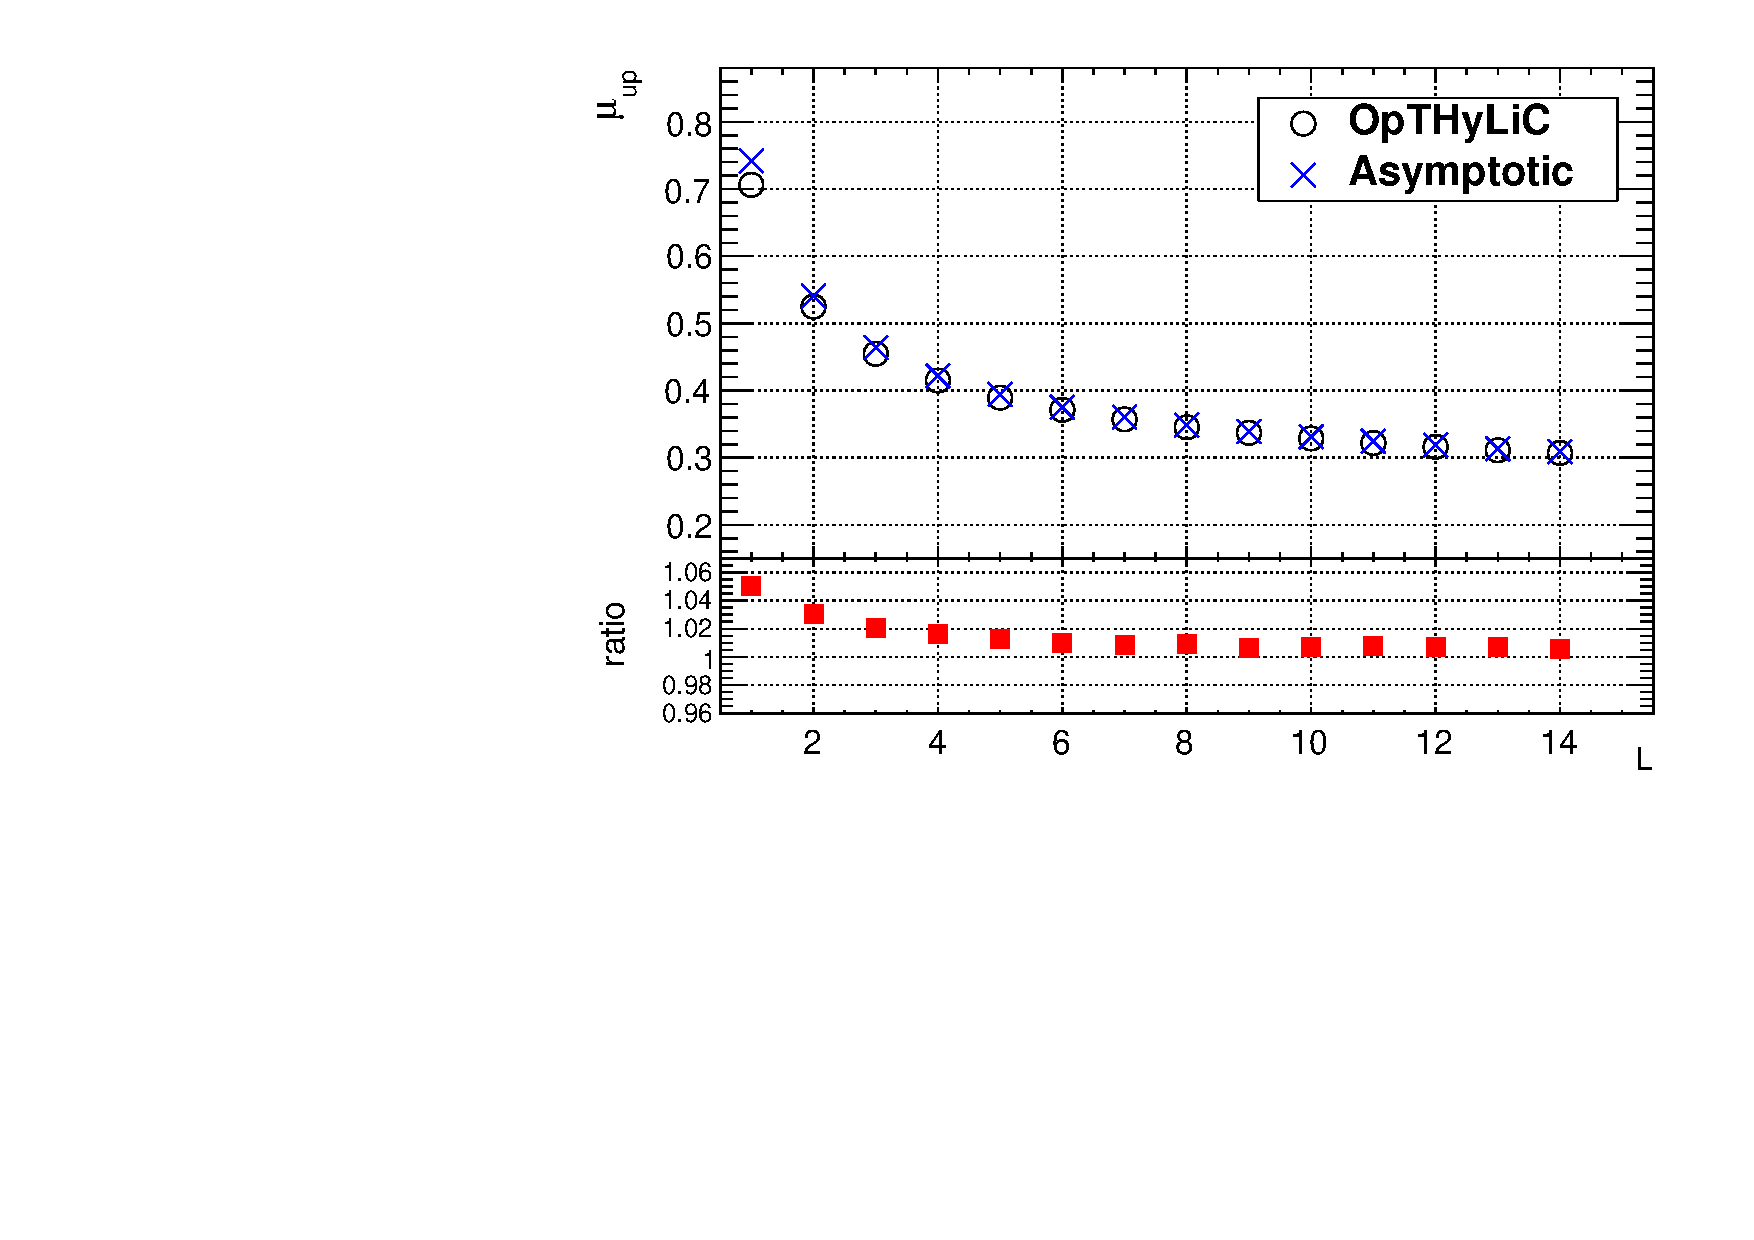
\includegraphics[scale=0.5]{figures/MultipleChannelsNoUncertainties_OTHVsAsymptotic.pdf}
\caption{Limite d'exclusion en fonction de $L$ calcul\'ee avec \opthylic~et \`a partir du r\'esultat asymptotique (\'equation~\ref{eq:CLsMultipleChannelsWoUncertAsympt}) pour la combinaison des trois canaux d\'efinis dans le texte. \label{fig:ThreeChannelExampleAsympt}}
\end{center}
\end{figure}

La figure~\ref{fig:ThreeChannelExampleAsympt} montre que, lorsque le nombre d'\'ev\'enements augmente, \opthylic~converge comme il se doit vers le r\'esultat asymptotique.

%\section{Calcul sur un canal avec incertitudes}
%\subsection{Calcul sur un canal avec incertitudes}
\subsection{Validation des calculs en pr\'esence d'incertitudes}
\label{sec:validOTHsyste}

Plusieurs \'etudes ont \'egalement \'et\'e r\'ealis\'ees pour valider le traitement des incertitudes statistiques et syst\'ematiques dans \opthylic~et \tifosi. 
Comme nous l'avons vu dans la section~\ref{sec:opthylic}, \opthylic~traite les incertitudes de mani\`ere bayésienne, par marginalisation. 
Une v\'erification simple de la proc\'edure de marginalisation a \'et\'e  r\'ealis\'ee en comparant la distribution marginale du nombre d'\'ev\'enements calcul\'ee par \opthylic{} \`a une solution analytique dans le cas o\`u il y a une seule source de bruit de fond.
Lorsque celle-ci est entach\'ee d'une incertitude statistique pour laquelle une distribution \prior~gamma est utilis\'ee, la distribution marginale 
%, donn\'ee par la distribution compos\'ee d'une distribution de Poisson et d'une distribution gamma, 
est binomiale n\'egative :
% (voir section~\ref{sec:OTHTreatmentStatUncerts}). 
%En effet, dans ce cas la distribution marginale, donn\'ee par la distribution compos\'ee d'une distribution de Poisson et d'une distribution gamma, est binomiale n\'egative :
\begin{equation}
\label{eq:NegativeBinomial}
\hspace*{-1cm}
\begin{split}
P(N=n|b^{\text{nom}},\sigma)&=\displaystyle\int_0^\infty P(N=n|b)\times f(b;b^{\text{nom}},\sigma)\dd b\\
 & =\frac{\Gamma\left(N+\left(\frac{b^{\text{nom}}}{\sigma}\right)^2\right)}{N!\Gamma\left(\left(\frac{b^{\text{nom}}}{\sigma}\right)^2\right)}\left(\frac{b^{\text{nom}}}{b^{\text{nom}}+\sigma^2}\right)^{\left(b^{\text{nom}}/\sigma\right)^2}\left(\frac{\sigma^2}{b^{\text{nom}}+\sigma^2}\right)^{N}
\end{split}
\end{equation}
o\`u $N$ est le nombre d'\'evenements observ\'e, $b$ le nombre d'\'ev\'enements de bruit de fond attendu, $b^{\text{nom}}$ sa valeur nominale, $\sigma$ son incertitude statistique, $P(N=n|b)$ la distribution de Poisson de param\`etre $b$, $f(b;b^{\text{nom}},\sigma)$ la distribution gamma pour $b$ d'esp\'erance $b^{\text{nom}}$ et d'\'ecart-type $\sigma$ (donn\'e par l'\'equation~\ref{eq:gammaPriorsInOTH}) et $P(N=n|b^{\text{nom}},\sigma)$ la distribution marginale (binomiale n\'egative) du nombre d'\'ev\'enements. La figure \ref{fig:SingleChannelStatUncertNegativeBinomial} montre que l'accord entre l'\'equation~\ref{eq:NegativeBinomial} et la distribution marginale calcul\'ee par \opthylic~est excellent lorsqu'une distribution \prior~$\pi\left(b\right)\propto 1/b$ est utilis\'ee ($\alpha=1$ dans l'\'equation~\ref{eq:gammaPriorsInOTH}). Un excellent accord a \'egalement \'et\'e trouv\'e pour les deux autres distributions \prior~disponibles dans \opthylic~($\pi\left(b\right)\propto 1$ et $\pi\left(b\right)\propto 1/\sqrt{b}$).

\begin{figure}[!htb]
\begin{center}
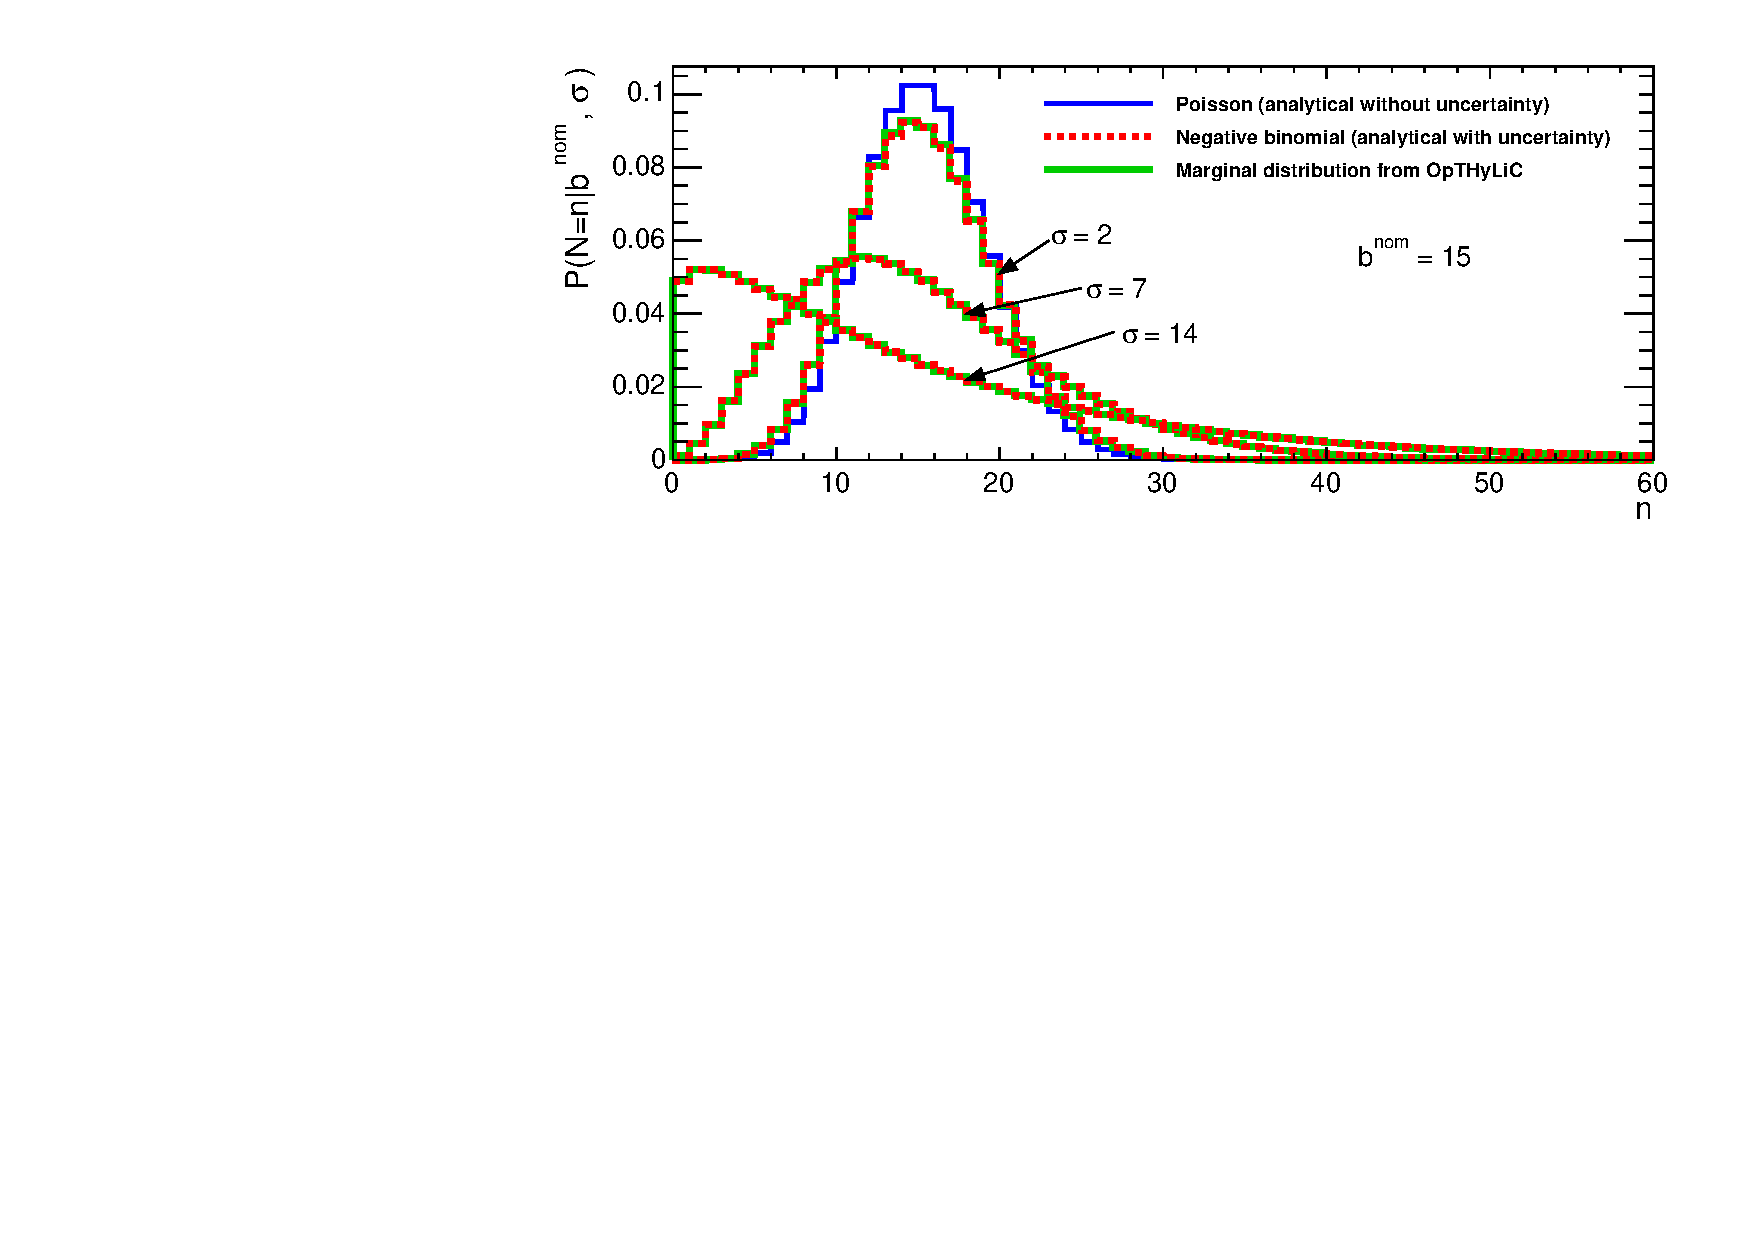
\includegraphics[scale=0.7]{figures/SingleChannelStatUncertNegativeBinomial.pdf}
\caption{Distribution marginale du nombre d'\'ev\'enements sous l'hypoth\`ese de bruit de fond dans le cas ou le bruit de fond a une incertitude statistique contrainte par une distribution gamma d'esp\'erance $b^{\text{nom}}=15$ et d'\'ecart-type $\sigma$ \'egal \`a $2, 7$ et $14$.\label{fig:SingleChannelStatUncertNegativeBinomial}}
\end{center}
\end{figure}

Pour la validation plus compl\`ete du traitement des incertitudes dans \opthylic~et \tifosi, le r\'esultat \'etabli dans la section~\ref{eq:equivalenceHybridBayesian} a \'et\'e utilis\'e. Plusieurs comparaisons entre les limites d'exclusion obtenues par ces deux outils
%\opthylic et par \tifosi~(d\'ecrit dans la section~\ref{sec:tifosi}) 
ont \'et\'e faites en changeant le nombre de sources de bruit de fond, le nombre d'incertitudes syst\'ematiques sur ces bruits de fonds et la valeur des nombres d'\'ev\'enements et des incertitudes. Un exemple avec les donn\'ees de la table~\ref{tab:ExampleValidUncert} est montr\'e sur la figure~\ref{fig:ExampleValidUncert}. 

\begin{table}[!htb]
\begin{center}
\begin{tabular}{c | c|c| c c c c c}
\hline\hline
\multirow{2}{*}{\'Echantillon}  &  nb \'ev\'enements   &   incertitude  & \multicolumn{5}{c}{incertitudes syst\'ematiques relatives}   \\
&  nominal  &   statistique  &  syst. 1 & syst. 2 & syst. 3 & syst. 4 & syst. 5 \\
\hline
Bruit fond 1 & $25\times L$  & $7$    &  $^{+0,1}_{-0,3}$   & $^{+0,3}_{-0,2}$  \\
\hline
Bruit fond 2 & $25\times L$  & $12$  &  $^{+0,2}_{-0,05}$  & & $^{-0,06}_{-0,15}$ \\
\hline
Bruit fond 3 & $33.3\times L$  & $3.5$    &  & $^{-0,1}_{+0,3}$ & $^{+0,15}_{-0,15}$  & $^{-0,6}_{+0,6}$  \\
\hline
Bruit fond 4 & $16.7\times L$  & $5$    &  & & & & $^{-0,3}_{+0,25}$ \\
\hline
Donn\'ees & $90\times L$   &  -  &  - & - & - & - & - \\
\hline
Signal & $5.0\times L$  &  $0$  & $^{0}_{0}$  & $^{0}_{0}$ & $^{0}_{0}$ & $^{0}_{0}$ &  $^{0}_{0}$\\
\hline
\end{tabular}
\end{center}
\caption{Exemple de configuration utilis\'ee pour valider le traitement des incertitudes statistiques et syst\'ematiques. Les incertitudes statistiques (syst\'ematiques) sont donn\'ees en absolu (relatif). Pour chaque incertitude syst\'ematique, un couple de valeur est donn\'e. La valeur du haut (bas) correspond \`a la variation relative sur le nombre d'\'ev\'enements lorsque la source de l'incertitude est vari\'ee de $+1\sigma$ ($-1\sigma$). Les incertitudes syst\'ematiques dans une m\^eme colonne sont consid\'er\'ees comme corr\'el\'ees \`a 100\%. Celles dans des colonnes diff\'erentes sont totalement d\'ecorr\'el\'ees. Les limites d'exclusion obtenues pour cette configuration sont montr\'ees sur la figure~\ref{fig:ExampleValidUncert}. \label{tab:ExampleValidUncert}}
\end{table}

\begin{figure}[!htb]
\begin{center}
\hspace*{-1.3cm}
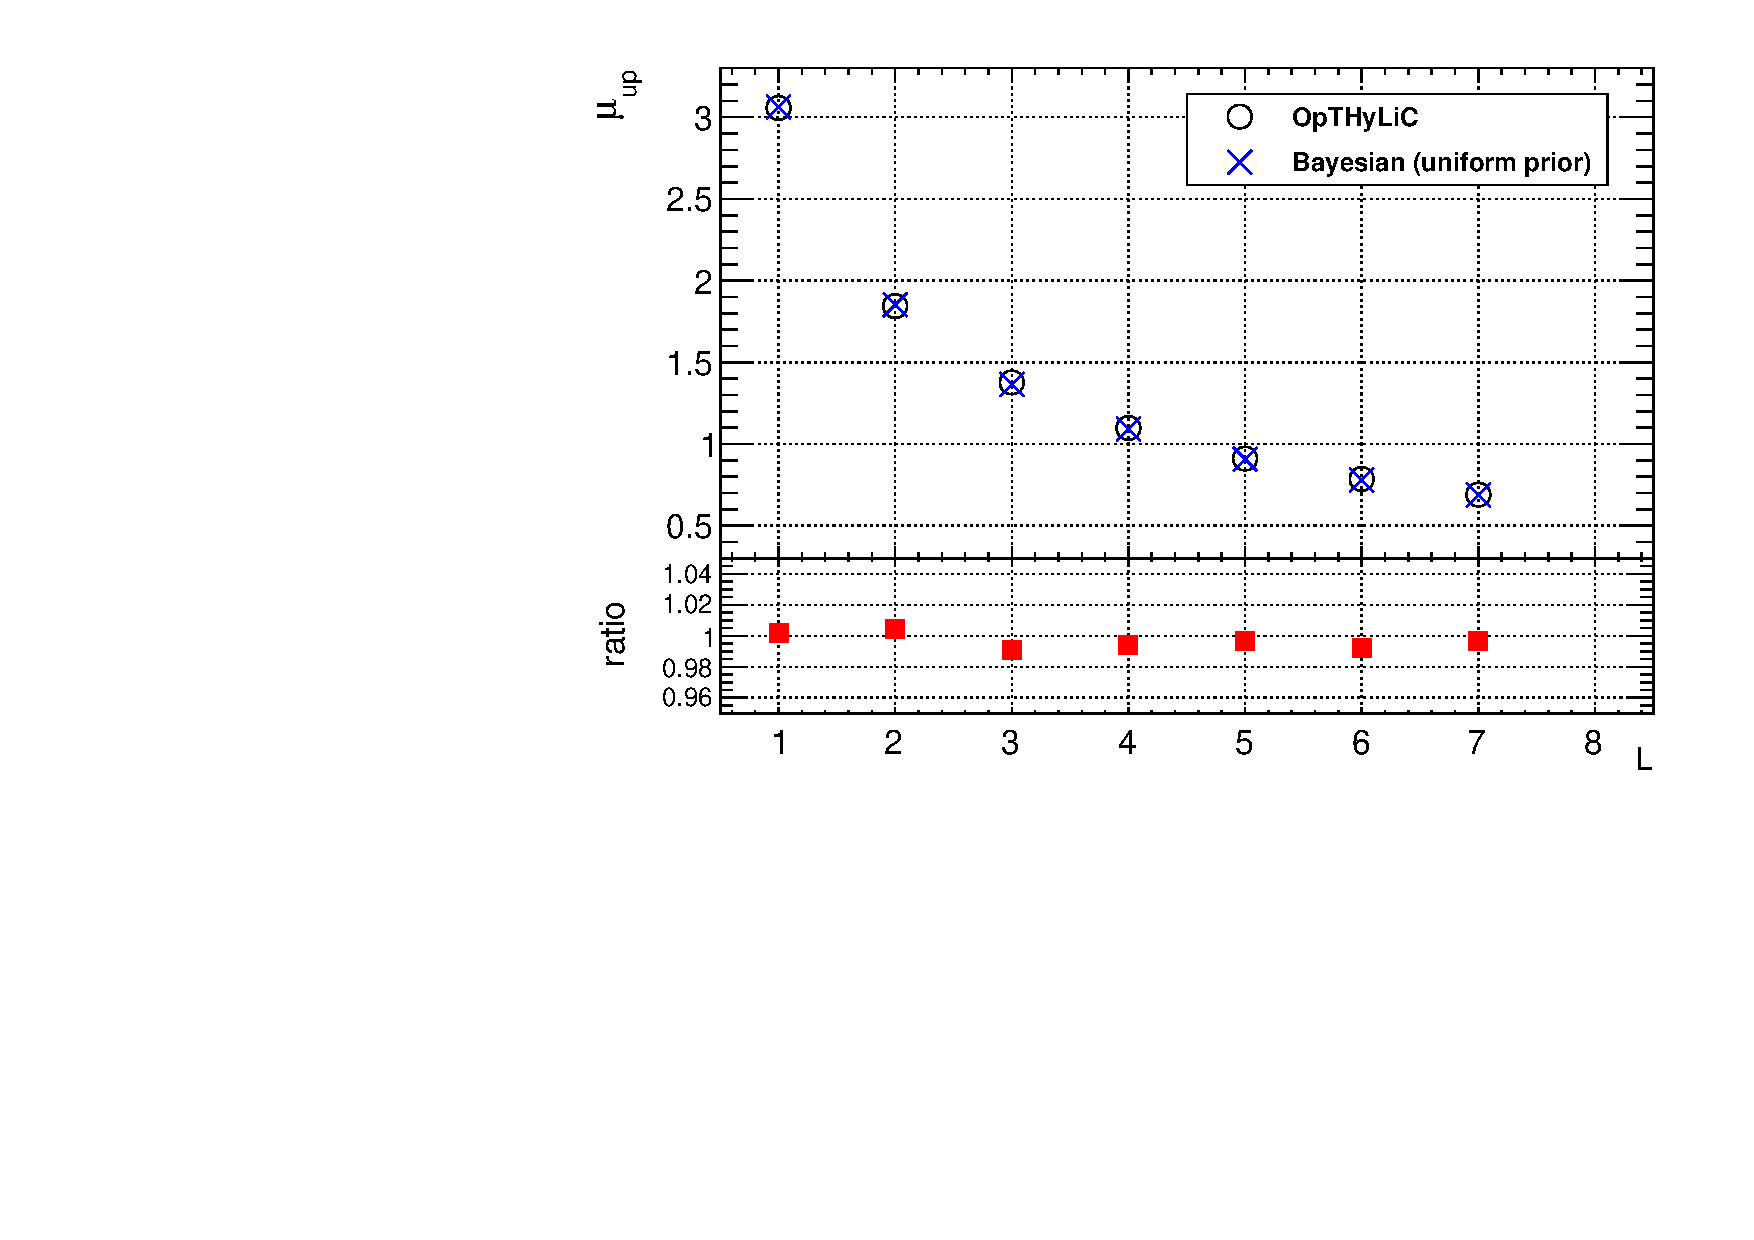
\includegraphics[scale=0.42]{figures/SingleChannelForComparisonWithUncertaintiesOnBkg.pdf}
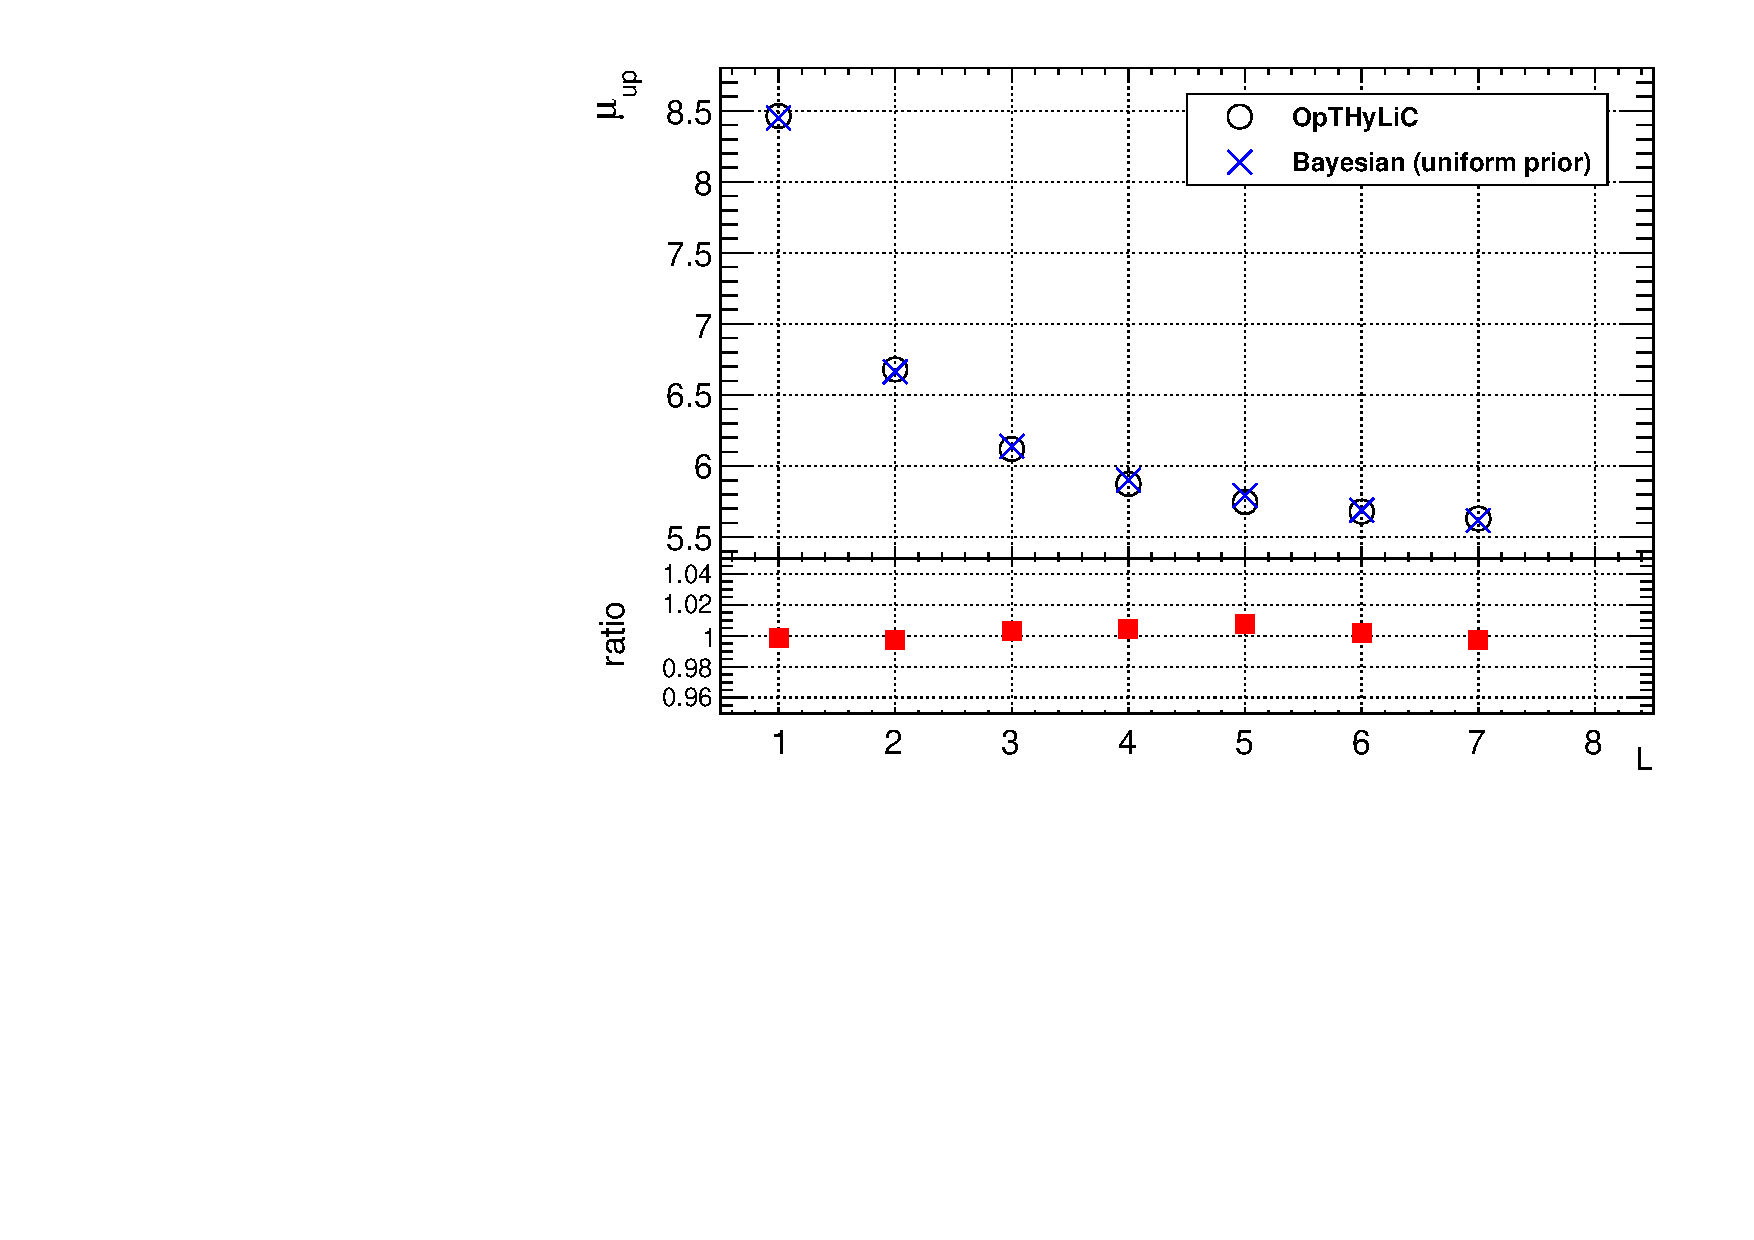
\includegraphics[scale=0.42]{figures/SingleChannelWithUncertaintiesOnBkg.pdf}
\caption{Limite d'exclusion en fonction de $L$ sans (\`a gauche) et avec (\`a droite) les incertitudes statistiques et syst\'ematiques. Une interpolation et extrapolation exponentielle a \'et\'e utilis\'ee pour les incertitudes syst\'ematiques et une contrainte normale a \'et\'e utilis\'ee pour les incertitudes statistiques.\label{fig:ExampleValidUncert}}
\end{center}
\end{figure}

L'exemple de la table~\ref{tab:ExampleValidUncert} a \'et\'e choisi car les incertitudes sont grandes et leur effet sur les limites d'exclusion est tr\`es prononc\'e (comme nous pouvons le voir en comparant les graphiques \`a gauche et \`a droite sur la figure~\ref{fig:ExampleValidUncert}). Ainsi, un mauvais traitement des incertitudes devrait \^etre visible. Un excellent accord a \'et\'e trouv\'e entre \opthylic~et \tifosi~. Il en est de m\^eme dans les autres cas test\'es. De mani\`ere rigoureuse, ces comparaisons ne valident que le traitement des incertitudes statistiques et syst\'ematiques pour les bruits de fond. Cependant, les incertitudes sur le signal sont trait\'ees par le m\^eme code que les incertitudes sur les bruits de fond et sont par cons\'equent indirectement valid\'ees par ce r\'esultat. 
%Les incertitudes sur le signal sont par cons\'equent suppos\'ees \^etre trait\'ees correctement. 

%Comme nous le verrons ci-dessous, la comparaison entre \mclimit~et \opthylic~montre que les incertitudes sur le signal sont effectivement trait\'ees correctement dans \opthylic.

%\section{Calcul sur plusieurs canaux avec incertitudes}
%\subsection{Calcul sur plusieurs canaux avec incertitudes}

Afin de s'assurer du traitement correcte des incertitudes (notamment celles sur le signal) et du calcul des limites attendues (\`a -2$\sigma$, -1$\sigma$, +1$\sigma$, +2$\sigma$ et m\'ediane) dans \opthylic, d'autres comparaisons ont \'et\'e faites mais cette fois-ci entre \opthylic~et \mclimit.
%Dans la derni\`ere validation que nous avons effectu\'ee, les limites d'exclusion observ\'ees et attendues (\`a -2$\sigma$, -1$\sigma$, +1$\sigma$, +2$\sigma$ et m\'ediane) calcul\'ees avec \opthylic~ont \'et\'e compar\'ees aux limites d'exclusion calcul\'ees avec \mclimit. 
\mclimit~est, comme \opthylic, un outil impl\'ementant l'approche hybride fr\'equentiste-bayesienne. Il utilise l'interpolation et l'extrapolation d\'ecrite dans la section~\ref{sec:OTHTreatmentSystUncerts} et des distributions \prior~gaussiennes pour les incertitudes statistiques. Lorsque \opthylic~est configur\'e de mani\`ere ad\'equat, il doit fournir les m\^emes limites observ\'ees et attendues que \mclimit. Pour cette comparaison, 
les donn\'ees de l'analyse de recherche du \english{sgluon} avec le lot de donn\'ees partiel mentionn\'e dans la section~\ref{sec:analyseFourTops} 
%des valeurs typiques pour les nombres d'\'ev\'enements attendus et observ\'es et leurs incertitudes 
ont \'et\'e utilis\'ees. La figure~\ref{fig:ExclusionPlot_Sgluon} montre une comparaison des limites d'exclusion en fonction de la masse obtenue en combinant les trois canaux leptoniques ($ee$, $e\mu$ et $\mu\mu$). Six valeurs de masse ont \'et\'e consid\'er\'ees et sept sources de bruit de fond sont pr\'esentes dans chaque canal. Le signal et les bruits de fond sont affect\'es par des incertitudes statistiques et syst\'ematiques. Pour chaque masse, le nombre total de param\`etres de nuisance est 51 (24 sont associ\'es \`a des incertitudes syst\'ematiques et 27 \`a des incertitudes statisques). Dans les deux cas, 50 000 pseudo-exp\'eriences sont utilis\'ees. Les limites obtenues par \opthylic~sont en bon accord avec celles trouv\'ees par \mclimit, validant ainsi les calculs. 
%\vspace*{-0.5cm}
%\enlargethispage{1cm}
\begin{figure}[!htb]
\begin{center}
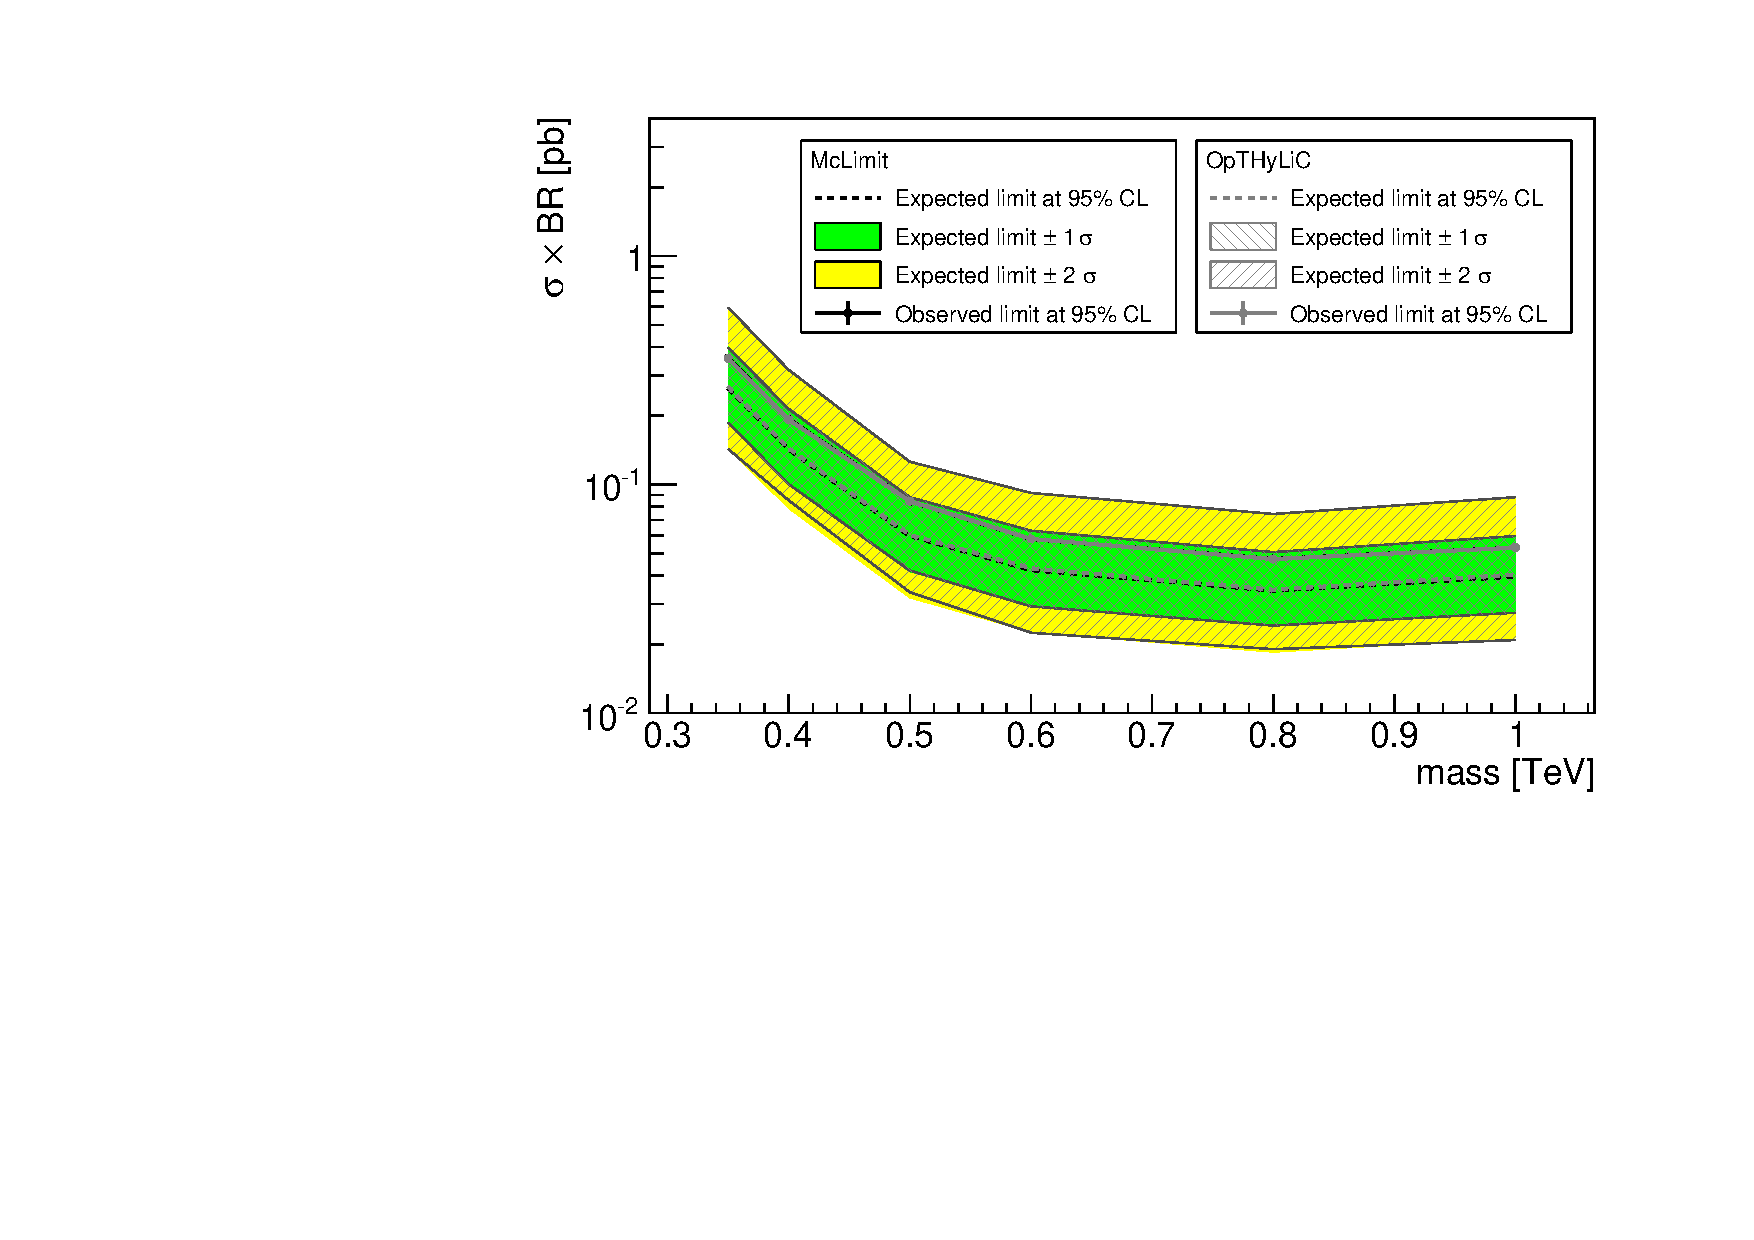
\includegraphics[scale=0.6]{figures/ExclusionPlot_Sgluon.pdf}
\caption{Comparaison des limites observées et attendues calculées avec \mclimit~et \opthylic~dans un cas réaliste (voir texte). \label{fig:ExclusionPlot_Sgluon}}
\end{center}
\end{figure} 

Cette comparaison illustre sur un exemple r\'ealiste une des diff\'erences principales entre \opthylic{} et \mclimit{}: le temps de calcul. Sur le m\^eme ordinateur, il a fallu 25 minutes (8 secondes) pour calculer la limite observ\'ee \`a 1~TeV avec \mclimit~(\opthylic). Le graphique complet est produit en moins de six minutes avec \opthylic~alors qu'il faut plusieurs heures pour le produire avec \mclimit.

%\section{Conclusion}
\subsection{Conclusion}

Les outils \opthylic~et \tifosi, impl\'ement\'es pour le calcul de limite 
d'exclusion sur les sections efficaces de production, ont \'et\'e 
pr\'esent\'es. Ces outils utilisent le m\^eme mod\`ele statistique et sont 
capables de prendre en compte un nombre arbitrairement grand de canaux et d'incertitudes 
statistiques et syst\'ematiques. 
Les corr\'elations entre ces derni\`eres sont \'egalement prises en compte. 
Les calculs r\'ealis\'es par ces outils ont \'et\'e valid\'es dans de nombreuses configurations, r\'ev\'elant un comportement toujours conforme aux attentes.
Quelques r\'esultats obtenus avec ces outils pour la recherche d'\'ev\'enements avec quatre quarks top sont pr\'esent\'es dans le chapitre suivant.

%Ils doivent par cons\'equent \^etre valid\'es avant de pouvoir \^etre utilis\'es dans une analyse de physique. Le chapitre suivant pr\'esente les \'etudes r\'ealis\'ees pour valider \opthylic.

%Les diff\'erentes \'etudes r\'ealis\'ees dans le but de valider l'outil 
%\opthylic~ont \'egalement \'et\'e pr\'esent\'ees. 
%\`A chaque fois, un tr\`es bon accord est observ\'e entre le r\'esultat attendu et le r\'esultat trouv\'e par \opthylic. 
%Cette outil est par cons\'equent valid\'e et peut \^etre utilis\'e pour 
%l'inf\'erence statistique dans la recherche de processus poissonniens. Quelques 
%r\'esultats obtenus dans la recherche d'\'ev\'enements avec quatre quarks top 
%dans l'\'etat final sont pr\'esent\'es dans le chapitre suivant.
